%!TEX root = ./main.tex
% arara: pdflatex
% arara: makeglossaries if changed('glo')
% arara: bibtex if changed(toFile('bibliographie.bib')) || changed('bcf')
% arara: pdflatex while changed('bbl') || changed('gls') || found('log', 'Please rerun') || found('log', 'Label(s) may have changed')

%%**************************************************************
%%
%% DHBW Heidenheim - Template for Bachelor Thesis
%%
%% Bevor usisng this template please have a look at the REAMDME.md file
%%
%%**************************************************************

%!TEX root = ../main.tex

% show warning for old LaTeX syntax
\RequirePackage[l2tabu, orthodox]{nag}

\documentclass[
	pdftex,
	oneside,
	14pt,			    % fontsize
	parskip=half,		    % Space (in lines) between paragraphs
	headheight = 12pt,    % Header hight
	headsepline,		    % Line after header
	footheight = 16pt,	    % Footer height
	footsepline,		    % Line before footer
	abstract=true,		    % Abstract headline
	DIV=calc,		    % Calculate print space
	BCOR=8mm,		    % BCOR settings (Bindekorrektur)
	headinclude=false,   % Exclude header from print space
	footinclude=false,	    % Exclude footer from print space
	listof=totoc,		    % Show List of Figures/Tables in Contents
	toc=bibliography,	    % Show Bibliography in Contents
]{scrreprt}	                     % Koma-Script report-class, long document: scrreprt, short document: scrbook

\usepackage{xstring}
\usepackage[utf8]{inputenc}
\usepackage[T1]{fontenc}

% iflang command definition
\newcommand{\iflang}[2]{%
	\IfStrEq{\documentLanguage}{#1}{#2}{}%
}

% ifDocType comand definition
\newcommand{\ifDocType}[3]{%
	\IfStrEq{\documentType}{#1}{#2}{#3}%
}

% ifMultipleAuthors definition
\newcommand{\ifMultipleAuthors}[2]{%
	\IfStrEq{\multipleAuthors}{true}{#1}{#2}%
}

% ifSpecialDocument definition
\newcommand{\ifSpecialDocument}[2]{\IfStrEqCase{\documentType}{%
		{T2_1000}{#2\ignorespaces}%
			{T2\_2000}{#2\ignorespaces}%
			{T2\_3100}{#2\ignorespaces}%
			{T2\_3300}{#2\ignorespaces}%
	}[#1\ignorespaces]%
}

% Include main settings
%!TEX root = ../main.tex

%% Citation Styles
% http://ctan.mirrorcatalogs.com/macros/latex/contrib/biblatex/doc/biblatex.pdf (3.3.1 Citation Styles)
% recommended:  z.B numeric-comp, alphabetic, 
% not recommended: authoryear, alphabetic-verb, 
\newcommand{\quoteStyle}{iso-numeric}

%% Fonts
%% palatino, goudysans, lmodern or libertine
\newcommand{\documentFont}{lmodern}

%% Margin
\newcommand{\margin}{2.5cm}

%% Space between chapter headline and top of page
\newcommand{\chapterMargin}{20pt}

%% Table settings
% Column spacing
\newcommand{\tableColumnMargin}{10pt}
%Line spacing
\newcommand{\tableRowMargin}{1.5}

%% Color settings
\newcommand{\defineColors}{%
	\definecolor{LinkColor}{HTML}{\linkColor}
	\definecolor{ListingBackground}{HTML}{F8F8F8}
}

%% Syntax Highlighting (Listings)
\newcommand{\listingsettings}{%
	\lstset{%
		language=Java,			% default language
		numbers=left,			% position of line numbers (left, right)
		stepnumber=1,			% set number to each line
		numbersep=5pt,			% 5pt between number and source code
		numberstyle=\tiny,		% letter size of numbers
		breaklines=true,		        % break lines if necessary (true, false)
		breakautoindent=true,	        % indenting after break line (true, false)
		postbreak=\space,		% break line after space
		tabsize=2,				% tabulator size
		basicstyle=\ttfamily\footnotesize, % font style
		showspaces=false,		% show space (true, false)		showstringspaces=false,	% show space in strings (true, false)
		extendedchars=true,		% show all Latin1 characters (true, false)
		captionpos=b,			% sets the caption-position to bottom
		backgroundcolor=\color{ListingBackground}, % source code background
		xleftmargin=10pt,		        % margin left
		xrightmargin=5pt,		        % margin right
		frame=single,			        % border settings
		frameround=ffff,
		rulecolor=\color{darkgray},	% border color
		fillcolor=\color{ListingBackground},
		aboveskip=20pt,
		keywordstyle=\color[rgb]{0.133,0.133,0.6},
		commentstyle=\color[rgb]{0.133,0.545,0.133},
		stringstyle=\color[rgb]{0.627,0.126,0.941}
	}
}


% Include document settings
%!TEX root = ../main.tex

%% Document language (en, de)
\newcommand{\documentLanguage}{de}

%% Document type
% T2\_1000 Project Thesis (Semester 1 & 2)
% T2\_2000 Project Thesis (Semester 3 & 4)
% T2\_3100 Seminar Paper (Semester 5 & 6)
% T2\_3300 Bachelor Thesis
\newcommand{\documentType}{T2\_3100}

\newcommand{\multipleAuthors}{false}
\newcommand{\documentAuthor}{Patrick Arndt}
\newcommand{\documentTitle}{Deep Learning auf medizinischen Bilddaten}
\newcommand{\documentPeriod}{5.&6. Semester}

\newcommand{\matriculationNumber}{7414700}

\newcommand{\locationUniversity}{Mosbach Campus Bad Mergentheim}
\newcommand{\department}{Angewandte Informatik}
\newcommand{\course}{INF20}

\newcommand{\degree}{Bachelor of Science}
% INF2014 - INF2016 (MI):       Bachelor of Science
% INF2014 - INF2016 (IA/IM) :   Bachelor of Engineering
% INF2017 (all):                Bachelor of Science

% A lecture that the document is written for
\newcommand{\lecture}{Software Engineering}
% Whether to show the lecture on cover
\newcommand{\showLecture}{false}

\newcommand{\releaseDate}{Mai 2023}
\newcommand{\releaseLocation}{Eckartshausen}

\newcommand{\companyName}{inevvo solutions GmbH \& Co. KG}
\newcommand{\companyLocation}{Waldzimmern}

\newcommand{\tutor}{Malte Tölle}
\newcommand{\evaluator}{Prof. Dr.\ Rolf Assfalg}

\newcommand{\linkColor}{00007A}


% Load language specific Strings
\input{lang/\documentLanguage}

% Load language specific babel package
\iflang{de}{\usepackage[english, ngerman]{babel}}
\iflang{en}{\usepackage[ngerman, english]{babel}}

% Add comment feature
\newcommand{\comment}[1]{\par {\bfseries \color{blue} #1 \par}}


%%%%%%% Package Includes %%%%%%%

\usepackage[margin=\margin,foot=1cm]{geometry}
\usepackage[activate]{microtype}
\usepackage[onehalfspacing]{setspace}
\usepackage{makeidx}
\usepackage[autostyle=true,german=quotes]{csquotes}
\usepackage{longtable}
\usepackage{enumitem}
\usepackage{graphicx}
\usepackage{pdfpages}
\usepackage{xcolor}
\usepackage{float}
\usepackage{array}
\usepackage{calc}
\usepackage[right]{eurosym}
\usepackage{wrapfig}
\usepackage{pgffor}
\usepackage[perpage, hang, multiple, stable]{footmisc}
\usepackage[printonlyused]{acronym}
\usepackage{listings}
\usepackage[obeyFinal,backgroundcolor=yellow,linecolor=black]{todonotes}
\usepackage{rotating}
\usepackage{lscape}
\usepackage{amsmath}
\usepackage{amssymb}
\usepackage{\documentFont}
\usepackage[%
	pdftitle={\documentTitle},
	pdfauthor={\documentAuthor},
	pdfsubject={\documentType},
	pdfcreator={pdflatex, LaTeX with KOMA-Script},
	pdfpagemode=UseOutlines,       % Show Contents while opening
	pdfdisplaydoctitle=true, 		% Show document title instead of file name
	pdflang={\documentLanguage}, % Document language
]{hyperref}
\usepackage{xurl}
\usepackage{bookmark}
\usepackage[nonumberlist,toc]{glossaries}
\usepackage{scrhack}
\usepackage{subcaption}
% Generate glossary
\makeglossaries{}

% Load colors
\defineColors{}

% Set Titel, Autor and Date
\title{\documentTitle}
\author{\documentAuthor}
\date{\datum}


% PDF link settings
\hypersetup{%
	colorlinks=true,
	linkcolor=LinkColor,
	citecolor=LinkColor,
	filecolor=LinkColor,
	menucolor=LinkColor,
	urlcolor=LinkColor,
	linktocpage=true,
	bookmarksnumbered=true
}

% Captions fontsize
\addtokomafont{caption}{\small}

% Bibliographie settings
\iflang{de}{%
	\usepackage[
		backend=bibtex,		% recommended. Alternative: bibtex
		bibwarn=true,
		bibencoding=utf8,	         % If .bib file is encoded with utf8, otherwise ascii
		%sortlocale=de_DE,
		shortnumeration=true,
		isbn=false,
		urldate=long,
		style=\quoteStyle,
	]{biblatex}
}
\iflang{en}{%
	\usepackage[
		backend=bibtex,		% recommended. Alternative: bibtex
		bibwarn=true,
		bibencoding=utf8,        % If .bib file is encoded with utf8, otherwise ascii
		sortlocale=en_US,
		style=\quoteStyle,
	]{biblatex}
}
\addbibresource{bibliographie.bib}

% Hurenkinder und Schusterjungen verhindern
% http://projekte.dante.de/DanteFAQ/Silbentrennung
\clubpenalty = 10000 % schließt Schusterjungen aus (Seitenumbruch nach der ersten Zeile eines neuen Absatzes)
\widowpenalty = 10000 % schließt Hurenkinder aus (die letzte Zeile eines Absatzes steht auf einer neuen Seite)
\displaywidowpenalty=10000

% Graphicspath
\graphicspath{{images/}}

% frequently used programing languages
\lstloadlanguages{PHP,Python,Java,C,C++,bash}

\listingsettings{}
% Rename Listings
\renewcommand\lstlistingname{\listingPhrase}
\renewcommand\lstlistlistingname{\listListingPhrase}
\def\lstlistingautorefname{\authorListingPhrase}

% Spaces in tables
\setlength{\tabcolsep}{\tableColumnMargin}
\renewcommand{\arraystretch}{\tableRowMargin}


%!TEX root = ../main.tex

%
% To create glossary run the following command: 
% makeglossaries main.acn && makeglossaries main.glo
%

%
% Glossareintraege --> referenz, name, beschreibung
% Aufruf mit \gls{...}
%
\newglossaryentry{Glossareintrag}{name={Glossareintrag},plural={Glossareinträge},description={Ein Glossar beschreibt verschiedenste Dinge in kurzen Worten}}
\newglossaryentry{Algorithmus}{name={Algorithmus},plural={Algorithmen},description={Ein Algorithmus ist eine genau definierte Folge von Aktionen, für die Lösung eines Problems\cite[vgl.][]{Algorithmus}}}
\newglossaryentry{Modell}{name={Modell},plural={Modelle},description={Ein Modell beschreibt eine komplexe mathematische Funktion, das anhand von Daten trainiert wurde, um bestimmte Vorhersagen oder Entscheidungen zu treffen. \cite[vgl.][]{MSModell}}}
\newglossaryentry{Ionisierende Strahlung}{name={Ionisierende Strahlung},description={Strahlung die so stark ist, das sie Elektronen aus Atomen oder Molekühlen entfernt kann, sodass diese positiv geladen sind (ionisiert). Diese Art von Strahlung kann Mensch und Umwelt schädigen.\cite[vgl.][]{IonisierendeStrahlung}}}
\newglossaryentry{Proton}{name={Proton},plural={Protonen},description={Ein stabiles, elektrisch positiv geladenes Teilchen.}}


\begin{document}

% Cover
\begin{spacing}{1}
  %!TEX root = ../main.tex

\begin{titlepage}
	\begin{longtable}{p{8cm} p{8cm}}
		\raggedright {\raisebox{\ht\strutbox-\totalheight}{
\includegraphics[height=2.5cm]{images/cover/logo-dhbw.pdf}}} &
	\end{longtable}
	\enlargethispage{20mm}
	\begin{center}
		\doublespacing{
			\vspace*{12mm}	{\LARGE\textbf \documentTitle }}\\
		\vspace*{12mm}	{\large\textbf {\documentTypePhrase}}\\
		
		% degre only for bachelor thesis
		\ifDocType{T2\_3300}{
			\vspace*{12mm}	\degreePhrase\\
			\vspace*{3mm}		{\textbf \degree}\\
		}
		
		\IfStrEq{\showLecture}{true}{
			\vspace*{12mm}	\lecturePhrase\\
			\vspace*{0mm}		{\textbf \lecture}\\
		}
		
		\vspace*{12mm}	\departmentPhrase{} \department\\
		\vspace*{0mm}		\locationUniversityPhrase{} \textbf{\locationUniversity}\\
		\vspace*{12mm}	\documentAuthorPhrase\\
		\vspace*{3mm}		{\large\textbf \documentAuthor}\\
		\vspace*{12mm}	\releaseDate\\
	\end{center}
	\vfill
	\begin{spacing}{1.2}
		\begin{center}
			\begin{tabbing}
				mmmmmmmmmmmmmmmmmmmmmmmm             \= \kill 
				\textbf{\matriculationNumberPhrase, \coursePhrase}  \>  \matriculationNumber, \course\\
				\textbf{\tutorPhrase}               \>  \tutor\\
			\end{tabbing}
		\end{center}
	\end{spacing}
\end{titlepage}



\end{spacing}
\newpage

\pagenumbering{Roman}

% Restriction notices
\ifDocType{T2\_3100}{%
  % no restricition notices for semester paper
}{%
  %!TEX root = ../main.tex

\thispagestyle{empty}

\section*{\restrictionNoticesPhrase}

\vspace*{2em}

\iflang{de}{%
Die vorliegende {\documentTypePhrase} mit dem Titel {\itshape{} \documentTitle{}\/} enthält
unternehmensinterne bzw. vertrauliche Informationen der {\companyName}, ist deshalb mit einem
Sperrvermerk versehen und wird ausschließlich zu Prüfungszwecken am Studiengang {\department}
der Dualen Hochschule Baden-Württemberg {\locationUniversity} vorgelegt. Sie ist ausschließlich zur
Einsicht durch den zugeteilten Gutachter, die Leitung des Studiengangs und ggf. den Prüfungsausschuss
des Studiengangs bestimmt.  Es ist untersagt,
\begin{itemize}
  \item den Inhalt dieser Arbeit (einschließlich Daten, Abbildungen, Tabellen, Zeichnungen usw.) als
        Ganzes oder auszugsweise weiterzugeben,
  \item Kopien oder Abschriften dieser Arbeit (einschließlich Daten, Abbildungen, Tabellen,
        Zeichnungen usw.) als Ganzes oder in Auszügen anzufertigen,
  \item diese Arbeit zu veröffentlichen bzw. digital, elektronisch oder virtuell zur Verfügung zu stellen.
\end{itemize}
Jede anderweitige Einsichtnahme und Veröffentlichung – auch von Teilen der Arbeit – bedarf der
vorherigen Zustimmung durch den Verfasser und {\companyName}.
}

%http://www.ib.dhbw-mannheim.de/fileadmin/ms/bwl-ib/Downloads_alt/Leitfaden_31.05.pdf

\iflang{en}{%
  The {\documentTypePhrase} on hand
  \begin{center}{\itshape{} \documentTitle{}\/}\end{center}
  contains internal resp.\ confidential data of {\companyName}. It is intended solely for inspection by the
  assigned examiner, the head of the {\department} department and, if necessary, the Audit
  Committee \locationUniversityPhrase{} {\locationUniversity}. It is strictly forbidden
  \begin{itemize}
    \item to distribute the content of this paper (including data, figures, tables, charts etc.) as a whole or
          in extracts,
    \item to make copies or transcripts of this paper or of parts of it,
    \item to display this paper or make it available in digital, electronic or virtual form.
  \end{itemize}
  Exceptional cases may be considered through permission granted in written form by the author
  and {\companyName}.
}

% \vspace{3em}

% \releaseLocation, \releaseDate
% \vspace{4em}

% \rule{6cm}{0.4pt}\\
% \documentAuthor

  \newpage
}%

% Declaration
%!TEX root = ../main.tex

\thispagestyle{empty}

\section*{\declarationPhrase}

\vspace*{2em}

\iflang{de}{%
  \ifMultipleAuthors{Wir versichern}{Ich versichere} hiermit, dass \ifMultipleAuthors{wir unsere}{ich meine}
  {\documentTypePhrase} mit dem Thema {\itshape \documentTitle }
  selbstständig verfasst und  keine anderen als die angegebenen Quellen und Hilfsmittel benutzt \ifMultipleAuthors{haben}{habe}.
}


\iflang{en}{%
  Hereby \ifMultipleAuthors{we}{I} solemnly declare:
  \begin{enumerate}
    \item that this {\documentTypePhrase}, titled {\itshape \documentTitle } is entirely the product of \ifMultipleAuthors{our}{my}
          own scholarly work, unless otherwise indicated in the text or references, or acknowledged below;
    \item \ifMultipleAuthors{we}{I} have indicated the thoughts adopted directly or indirectly from other sources at the appropriate
          places within the document;
    \item this {\documentTypePhrase} has not been submitted either in whole or part, for a degree at this or
          any other university or institution;
    \item \ifMultipleAuthors{we}{I} have not published this {\documentTypePhrase} in the past;
    \item the printed version is equivalent to the submitted electronic one.
  \end{enumerate}
  \ifMultipleAuthors{We are}{I am} aware that a dishonest declaration will entail legal consequences.
}

\vspace{3em}

\releaseLocation, \releaseDate
\vspace{4em}

\rule{6cm}{0.4pt}\\
\documentAuthor

\newpage

% Abstract
%!TEX root = ../main.tex

\pagestyle{empty}

% override abstract headline
\renewcommand{\abstractname}{Abstract}

\begin{abstract}

\end{abstract}
\newpage

% only page number in footer
\pagestyle{plain}

% space bevore chapter headline
\RedeclareSectionCommand[beforeskip=\chapterMargin]{chapter}

% Contents
\begin{spacing}{1.1}
\begingroup

% set subchapter depth
\setcounter{tocdepth}{3}
\setcounter{secnumdepth}{3}

\tableofcontents
\clearpage
\endgroup
\end{spacing}
\newpage

%!TEX root = ../main.tex

%
% To create glossary run the following command: 
% makeglossaries main.acn && makeglossaries main.glo
%

%
% Glossareintraege --> referenz, name, beschreibung
% Aufruf mit \gls{...}
%
\newglossaryentry{Glossareintrag}{name={Glossareintrag},plural={Glossareinträge},description={Ein Glossar beschreibt verschiedenste Dinge in kurzen Worten}}
\newglossaryentry{Algorithmus}{name={Algorithmus},plural={Algorithmen},description={Ein Algorithmus ist eine genau definierte Folge von Aktionen, für die Lösung eines Problems\cite[vgl.][]{Algorithmus}}}
\newglossaryentry{Modell}{name={Modell},plural={Modelle},description={Ein Modell beschreibt eine komplexe mathematische Funktion, das anhand von Daten trainiert wurde, um bestimmte Vorhersagen oder Entscheidungen zu treffen. \cite[vgl.][]{MSModell}}}
\newglossaryentry{Ionisierende Strahlung}{name={Ionisierende Strahlung},description={Strahlung die so stark ist, das sie Elektronen aus Atomen oder Molekühlen entfernt kann, sodass diese positiv geladen sind (ionisiert). Diese Art von Strahlung kann Mensch und Umwelt schädigen.\cite[vgl.][]{IonisierendeStrahlung}}}
\newglossaryentry{Proton}{name={Proton},plural={Protonen},description={Ein stabiles, elektrisch positiv geladenes Teilchen.}}

\printglossary[style=altlist,title=\glossaryPhrase]

% Acronyms
\cleardoublepage
%!TEX root = ../main.tex

\addchap{\acronymsPhrase}

\begin{acronym}[YTMMM]
\setlength{\itemsep}{-\parsep}

\acro{AGPL}{Affero GNU General Public License}
\acro{BraTS}{Brain Tumor Segmentation Challenge}
\acro{CNN}{Convolutional Neural Network}
\acro{GPU}{Graphics Processing Unit}
\acro{KI}{Künstliche Intelligenz}
\acro{KNN}{Künstliches Neuronales Netz}
\acro{MRT}{Magnetresonanztomographie}
\acro{ReLU}{Rectified Linear Unit}
\acro{SGD}{Stochastic Gradient Descent}
\end{acronym}


% List of Figures
\cleardoublepage
\listoffigures

%List of Tables
\cleardoublepage
\listoftables

% List of Listings
\cleardoublepage
%\lstlistoflistings
%\cleardoublepage

\pagenumbering{arabic}

\pagestyle{headings}

% Content
%!TEX root = ../../main.tex

\chapter{Einleitung}
\section{Einführung und Hintergrund}
In der Medizin gibt es schon seit mehr als 50 Jahren bildgebende Verfahren, mit denen Aufnahmen vom Inneren des menschlichen Körpers möglich sind. Diese Verfahren wurden kontinuierlich weiterentwickelt und sind inzwischen in der Lage detaillierte Bilder zu erzeugen. Technologien wie eine Computertomographie (CT) oder eine \ac{MRT} sind in der Lage präzise Informationen über innere Organe, Strukturen und Gewebe im Körper zu liefern. \cite[vgl.][]{Heinrichs2022} Mit den modernen bildgebenden Verfahren, steigt die Datenmenge und Komplexität, wie auch die Herausforderung der Analyse und Verarbeitung der Daten bzw. Bilder. 

Aufgrund der immer weiter fortschreitenden Technologien, setzen immer mehr medizinische Institutionen auf bildgebende Verfahren, um so Krankheiten zu diagnostizieren und behandeln. Allerdings ist die Analyse und Verarbeitung dieser Daten mit der Zeit komplexer geworden, sodass Ärzte und Mediziner vor eine Herausforderung gestellt werden. Die manuelle Analyse und Verarbeitung der Daten bringt oft Schwierigkeiten und Fehlerquellen mit sich. Der Prozess ist meist sehr zeitintensiv, weshalb es häufig zu langen Wartezeiten bei Auswertungen für die Patienten kommen kann. Nicht nur die Wartezeit ist ein Problem, sondern auch menschliche Fehler bei Interpretation der Daten, welche zu Fehldiagnosen oder -behandlungen führen können. \cite[vgl.][]{Ramsundar2020}

Diese Herausforderungen können mithilfe des vielversprechenden Ansatzes der Automatisierung gelöst werden. So kann bspw. die Effizienz gesteigert und die Fehlerrate gesenkt werden. Ein wichtiges Stichwort ist hierbei \ac{KI}, die ebenfalls in den vergangenen Jahren enorme Fortschritte gemacht hat. Insbesondere im Bereich der Bildanalyse haben \ac{KI}-Systeme durch die Entwicklung von Deep Learning-\gls{Modell}en enorm an Genauigkeit gewonnen. Die Anwendung von Deep Learning auf medizinische Bilddaten bietet vielversprechende Möglichkeiten für eine verbesserte Diagnose, Therapieplanung und -überwachung sowie für die Entwicklung von personalisierten Medizinlösungen. 

Besonders im medizinischen Bereich hat die Nutzung von \ac{KI}-Systemen auf medizinischen Bilddaten in den letzten Jahren an Bedeutung gewonnen. Mithilfe von Deep Learning-Modellen können Ärzte und Forscher komplexe Bilder von medizinischen Bildgebungsverfahren wie Röntgenaufnahmen, CT-Scans und MRT-Scans automatisiert analysieren. Diese Analyse kann zur Erkennung von Krankheiten, Identifizierung von Tumoren, sowie zur Bewertung der Therapieeffektivität eingesetzt werden. 


\section{Problemstellung und Zielsetzung}
Die zunehmende Komplexität und Menge an medizinischen Daten und Bildern stellt Mediziner vor große Herausforderungen. Die manuelle Analyse und Verarbeitung der Daten ist zeitaufwendig, fehleranfällig und es besteht die Gefahr wichtige Sachen zu übersehen, welche für die Diagnose nützlich sind.
Gerade im Bereich der Tumore, also der Krebszellen, ist die frühzeitige Erkennung aber auch die Behandlung sehr wichtig für das Wohl des Patienten. 

Vor allem im Bereich des Gehirns ist mit Tumoren sehr behutsam umzugehen, um so keine bleibenden Schäden beim Patienten zu hinterlassen. Bei Gehirntumoren ist es wichtig die genaue Position und Lage zu kennen, damit eine geeignete Behandlung gefunden werden kann. Die Operation bei einem Gehirntumor bedarf großer Vorbereitung und ist komplex, da Fachärzte zunächst den Tumor genau segmentieren müssen, bevor sie weitere Schritte planen. Diese Vorbereitung ist unter anderem zeitintensiv und kann nur von ausgebildeten Fachärzten übernommen werden. 

Befindet sich ein Tumor im Gehirn, so bedarf es einer noch genaueren Vorbereitung und Arbeit, um diesen zu entfernen. 
Krebs ist ein vielseitiges Thema, mit dem sich die Medizin seit Jahren beschäftigt. Heutzutage setzen Ärzte vor allem bei der frühzeitigen Erkennung von Tumoren auf die Hilfe von \ac{KI}. Doch nicht nur bei der Früherkennung, sondern auch bei der Behandlung solcher Tumore. Sind solche im Bereich des Gehirns, ist es wichtig behutsam vorzugehen, um so keine bleibenden Schäden zu verursachen.

Die Problemstellung dieser Studienarbeit ist die Identifizierung und Klassifizierung von Tumoren im Gehirn. Die verwendeten Daten sind aus dem öffentlichen Datensatz BraTS (Brain Tumor Segmentation Challenge), welcher aus rund 1250 \ac{MRT}-Bildern von Gehirnen besteht, welche von Fachärzten auf Tumore untersucht und wenn vorhanden markiert wurden. Eine Herausforderung dabei ist es, ein geeignetes Deep Learning \gls{Modell} zu entwickeln, dass für die Segmentierung von Tumoren im Gehirn geeignet ist und möglichst genaue Ergebnisse liefert.  

Die Zielsetzung dieser Arbeit ist die Erstellung eines \gls{Modell}s für die Segmentierung von Gehirntumoren, anhand des BraTS Datensatzes. Das \gls{Modell} soll in der Lage sein zwischen drei verschiedenen Tumor-Klassen zu unterscheiden und für diese eine Maske zu erstellen. Für die Entwicklung des Modells wird das Open Source Machine-Learning Framework PyTorch verwendet, welches von Facebook entwickelt wurde. Das Framework bietet zahlreiche Tools und Funktionen für das Entwickeln von Deep Learning-\glspl{Modell}. \cite[vgl.][]{PyTorch}
%!TEX root = ../../main.tex
\chapter{Theoretische Grundlagen}
\section{Künstliche Intelligenz}
\ac{KI} wird zunehmend in verschiedenen Bereichen eingesetzt und erleichtert die Arbeit der Menschen enorm. Viele Arbeiten können mit Hilfe von \ac{KI} schneller und besser erledigt werden. Im folgenden Abschnitt werden die Begriffe 'Intelligenz' und 'Künstliche Intelligenz' erläutert, um ein einfaches Verständnis zu schaffen. Außerdem werden die verwandten Begriffe Machine Learning und Deep Learning in den Kontext eingeordnet.

In der Psychologie bezieht sich Intelligenz auf die Fähigkeit, logische, sprachliche, mathematische oder sensorische Probleme zu lösen, aber es gibt keine allgemeingültige Definition von Intelligenz. Die kognitiven Fähigkeiten des Menschen ermöglichen es ihm, sich an Beschreibungen oder Erklärungen von Dingen zu erinnern, die er zu einem späteren Zeitpunkt wieder abrufen und verwenden kann. Das menschliche Gehirn, das aus Milliarden von Neuronen besteht, lernt und speichert bestimmte Strukturen, Konzepte und Fähigkeiten. Beim Lernen werden die Verbindungen zwischen den Neuronen im Gehirn verstärkt. Je öfter etwas gelernt wird, desto stärker werden bestimmte Verbindungen zwischen den Neuronen im Gehirn. \cite[vgl.][]{Ertel2021,Posthoff2022}

Künstliche Intelligenz hingegen ist ein Wissenschaftsgebiet, das sich damit beschäftigt, Computern menschliches Verhalten beizubringen. Damit ist gemeint, dass ein Computer darauf trainiert wird, ähnlich wie ein Mensch zu denken und entsprechend zu handeln. \cite[vgl.][]{Lang2023} Im Gegensatz zu biologischen Neuronen lösen Computer Probleme wie die Klassifizierung eines Bildes durch die Anwendung mathematischer Funktionen und Algorithmen. Es wird versucht, die Denkfähigkeit des Menschen nachzuahmen, um einen Mehrwert bei der Problemlösung durch Computer zu erzielen. Mit Hilfe der künstlichen Intelligenz sind Computer heute in der Lage, Probleme zu lösen, die früher ein höheres intellektuelles Verständnis erforderten. Computer können beispielsweise Bilder klassifizieren oder Vorhersagen treffen. Ähnlich wie der Mensch lernt auch der Computer aus den vorhandenen Daten und verstärkt dabei bestimmte mathematische Zusammenhänge. \cite[vgl.][]{WasIstKi}

\begin{figure}[h]
	\centering
	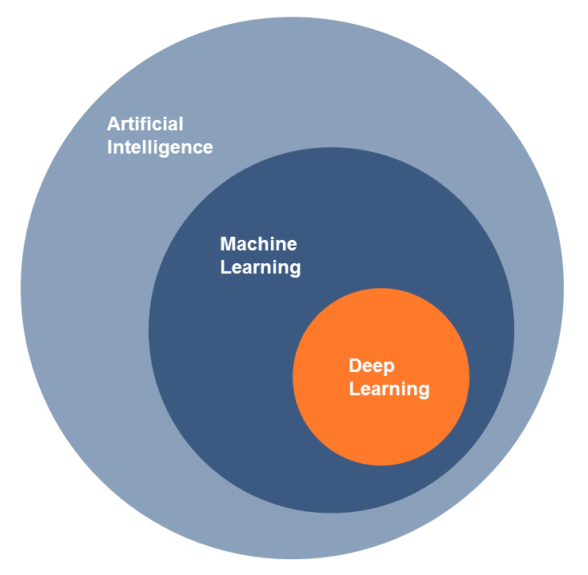
\includegraphics[height=.7\textwidth]{ai_overview.png}
	\caption{Übersicht der Bereiche von künstlicher Intelligenz (Quelle: \url{https://www.alexanderthamm.com/de/blog/ki_artificial-intelligence-ai-kuenstliche-neuronale-netze-machine-learning-deep-learning/})}
\end{figure}

Im Zusammenhang mit \ac{KI} wird häufig auch von Machine Learning, Deep Learning und Neuronalen Netzen gesprochen. \ac{KI} ist der Oberbegriff, der sowohl Machine Learning als auch Deep Learning umfasst. Deep Learning ist ein Teilbereich des Machine Learning, bei dem künstliche neuronale Netze zum Einsatz kommen, die es Computern ermöglichen, Dinge zu lernen und Probleme zu lösen. Im Folgenden wird der Schwerpunkt auf den Bereich Deep Learning gelegt.
%!TEX root = ../../main.tex
\section{Deep Learning}
\subsection{Einführung}
Viele Probleme oder Aufgaben können heutzutage mit einem Computer effizient gelöst werden. Dazu wird in der Regel ein \gls{Algorithmus} verwendet, der die Aufgabe systematisch löst. Es gibt jedoch komplexe Aufgaben, bei denen ein \gls{Algorithmus} nicht im Stande ist diese zu lösen.

Ein Beispiel dafür ist, vorherzusagen was ein Kunde in nächster Zeit kaufen wird, um ihm passende Vorschläge zu unterbreiten. Probleme dieser Art können nicht mit einem Algorithmus gelöst werden, sondern die Lösung muss anhand von vorhandenen Daten bestimmt werden. In solchen Fällen soll der Computer selbst einen Algorithmus erstellen, welcher dann auf neue Daten angewendet werden kann. Der Computer lernt mithilfe bereits vorhandener Daten oder Erfahrungen einen Algorithmus zu extrahieren, hierbei werden unter anderem Muster und Strukturen erkannt. Mit dem extrahierten Algorithmus kann anschließend das Kaufverhalten des Kunden approximiert werden. Möglich wird dies durch die enormen Datenmengen, die sich in den letzten Jahren angesammelt haben. Bei jedem Online Einkauf, Webseitenaufruf oder  beim Öffnen einer App werden Daten produziert und gesammelt. Diese Daten können letztendlich dazu verwendet werden, um Probleme wie oben beschrieben zu lösen.\cite[vgl.][]{Alpaydin2014}

Aufgaben wie das Klassifizieren von Bildern, komponieren von Musik\footnote{siehe \cite{GoogleMusicLM} } oder auch das erzeugen von Daten anhand eines Textes sind heutzutage mit Deep Learning möglich. Es gibt drei verschiedene Hauptarten wie ein Computer lernen kann, diese sind in den Abschnitten \ref{sec:ÜberwachtesLernen}, \ref{sec:UnüberwachtesLernen} und \ref{sec:BestärkendesLernen} beschrieben.


\subsection{Überwachtes Lernen}
\label{sec:ÜberwachtesLernen}
Überwachtes Lernen ist ein wichtiger Bereich des maschinellen Lernens, bei dem ein \gls{Modell} anhand von beschrifteten (oder ``gelabelt'') Daten lernt. Beschriftet bedeutet, dass den Daten bereits das gewünschten Ergebnis oder der erwartete Wert zugeordnet ist. Ziel des überwachten Lernens ist es, einen \gls{Algorithmus} oder ein \gls{Modell} zu finden, welches für neue und ungesehene Daten die richtigen Beschriftungen liefert.\cite[vgl.][]{Frochte2020,IBMSupervisedLearning} \\
Das Überwachte Lernen beinhaltet zwei verschiedene Problemstellungen, die Klassifikation und die Regression. Bei einer Klassifikation bekommen Bilder eine oder auch mehrere Klassen zugeordnet, es können aber auch Texte, Videos oder andere Dinge klassifiziert werden. Ein Beispiel dafür wäre die Klassifizierung von Hunden und Katzen auf Bildern. Dabei wird eine große Anzahl an Bildern von Hunden und Katzen in das \gls{Modell} gereicht und dieses fügt den Bildern jeweils die richtigen Klassen hinzu. Sieht das \gls{Modell} z.B. ein Bild mit einem Hund, so kann es nach dem Training die Klasse ``Hund'' zuordnen. In den meisten Email Programmen wird ein solches Klassifikationsmodell verwendet, um von seriösen und Spam Emails zu unterscheiden. Das Ergebnis einer Klassifikation ist immer eine Kategorie, welche die zu klassifizierenden Daten am besten beschreibt. \\
Die zweite Problemstellung, die es beim Überwachten Lernen gibt ist die Regression, diese wird oft für Vorhersagen und Prognosen verwendet.  Sie ist ähnlich zur Klassifizierung, jedoch ist hier die Zielmenge eine andere. Es wird versucht Werte für einen meist kontinuierlichen Bereich vorherzusagen,dazu wird der Datensatz mittels einer Funktion approximiert. Das Ergebnis einer Regression sind Werte bzw. Punkte, welche am besten die Funktion beschreiben.\cite[vgl.][]{Frochte2020} \\
Die Studienarbeit befasst sich nachfolgend hauptsächlich mit dem Überwachten Lernen, genauer gesagt mit der Klassifikation. Hierbei wird jedoch kein komplettes Bild klassifiziert, wie im oben genannten Beispiel, sondern es werden Klassen auf die einzelnen Pixel im Bild zugewiesen.

\subsection{Unüberwachtes Lernen}
\label{sec:UnüberwachtesLernen}
Beim Unüberwachten Lernen besitzen Daten keine Beschriftungen oder Kategorien, wie es beim Überwachten Lernen der Fall ist. Diese Methode des maschinellen Lernens kommt zum Einsatz, wenn das Beschriften der Daten nicht ohne weiteres möglich ist. Das \gls{Modell} sucht innerhalb der Daten, ohne vorgegebene Kategorien, nach Mustern und Strukturen. Anhand von statistischen Methoden wird die beste Kategorisierung der Daten gebildet. Die Ergebnisse des Unüberwachten Lernens sind verschiedene Gruppen von Daten, die allerdings keine Bezeichnung besitzen, sondern durchnummeriert werden. Die verschiedenen Daten in den Gruppen haben ähnliche oder die gleichen Eigenschaften.\\
Ein gutes Beispiel ist der Teil ``Kunden kauften auch'' auf Amazon. Hier werden dem Kunden ähnliche Produkte vorgeschlagen oder Artikel die oft in Kombination gekauft werden. Es wird dabei keine bestimmte Kategorie von Produkten genannt, sondern nur ähnliche Produkte vorgeschlagen. Es ist schwierig die Ergebnisse des Unüberwachten Lernens zu beurteilen, da keine vergleichbaren Daten mit entsprechenden Beschriftungen vorliegen und so auch kein Fehler berechnet werden kann.\cite[vgl.][]{Lang2023,Frochte2020}


\subsection{Bestärkendes Lernen}
\label{sec:BestärkendesLernen}
Es gibt oft Probleme, bei denen nicht genau bestimmt werden kann, ob etwas richtig oder falsch ist. Die Daten bei derartigen Problemen, insofern welche vorliegen, besitzen deshalb keine Beschriftungen. Es ist allerdings möglich zu sagen, ob Ergebnisse geeignet oder ungeeignet für die Lösung des Problems sind, in diesen Fällen kommt das Bestärkte Lernen zum Einsatz.Im Bereich der Robotik ist Bestärktes Lernen ein klassischer Anwendungsfall. Für Roboter sind in der Regel keine Trainingsdaten verfügbar, daher muss dieser eigenständig lernen, was gut und schlecht ist. \cite[vgl.][]{Ertel2021} \\
Das Ziel des Roboters ist es eine geeignete Lösung bzw. Strategie für das Problem zu finden. Beim Bestärkten Lernen ist oft die Rede von sogenannten Agenten, die für eine Lösung eines Problems trainiert werden. Bei der Suche nach einer geeigneten Strategie, werden diese kontinuierlich belohnt oder bestraft für gute und schlechte Aktionen. Ein einfaches Beispiel wäre ein Saugroboter,dieser saugt in einem Hotel die Zimmer. In den Zimmern, in welchen der Roboter z.B. nichts umgestoßen hat, wird er belohnt. Stößt der Roboter Dinge um, oder saugt etwas nicht gewolltes ein, so wird er bestraft. \cite[vgl.][]{Frochte2020} Das Belohnungssystem kann auf Punkten basieren, so würde der Saugroboter im positiven Fall Pluspunkte und im negativen Fall Minuspunkte bekommen und anhand dessen seine Aktionen anpassen.

\subsection{Künstliches Neuronales Netz (\acs{KNN})}
Die Struktur und Funktion des menschlichen Gehirns ist das Vorbild der künstlichen Neuronalen Netze. Sie besitzen eine Vielzahl künstlicher Neuronen, die miteinander verbunden sind und Informationen verarbeiten. Ein \ac{KNN} wird für verschiedene Anwendungen eingesetzt, wie z.B. Mustererkennung, Datenanalyse oder Vorhersagen.

\subsubsection{Biologisches Neuron}

\begin{figure}[h]
	\centering
	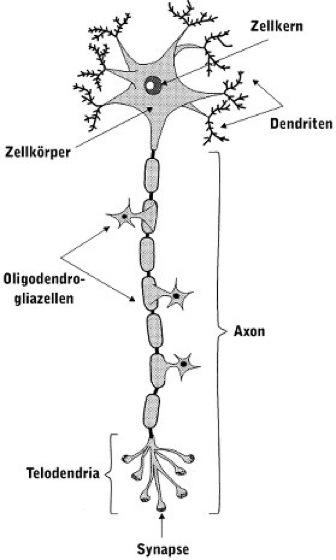
\includegraphics[width=.4\textwidth]{biologisches_neuron.jpg}
	\caption{Aufbau biologisches eines biologischen Neurons (Quelle: \url{https://www.spektrum.de/lexikon/psychologie/neuron/10516})}		\label{fig:BioNeuron}
\end{figure}

Das biologische Neuron (siehe Abb. \ref{fig:BioNeuron}) ist das Vorbild der künstlichen Neuronen. Es besteht aus Dendriten, welche die elektrischen Signale der anderen Neuronen entgegen nehmen und diese an den Zellkörper weiterleiten. 
Am Axonhügel, der zwischen dem Zellkörper und Axon liegt, werden die elektrischen Signale gesammelt und summiert. Erst beim Überschreiten eines gewissen Schwellenwertes, wird das Signal weiter an das Axon geleitet. Durch den Schwellenwert wird verhindert, das sehr kleine Signale weitergeleitet werden, die keine Relevanz haben. Ohne das Filtern der Signale, wäre eine Verarbeitung der relevanten Signale nicht möglich. Das Signal welches letztendlich über das Axon an die Synapsen transportiert wird, heißt Aktionspotential. An die Synapsen schließen andere Dendriten von Neuronen an und empfangen die weitergeleiteten Signale. Ein biologisches Neuron kann dabei bis zu mehreren tausend Verbindungen zu anderen Neuronen besitzen, diese können wieder dementsprechend viele Verbindungen haben.\cite[vgl.][]{Posthoff2022,JuergenCleve2020}

\subsubsection{Künstliches Neuron}
\label{subsubsec:KünstlichesNeuron}
\begin{figure}[ht]
	\centering
	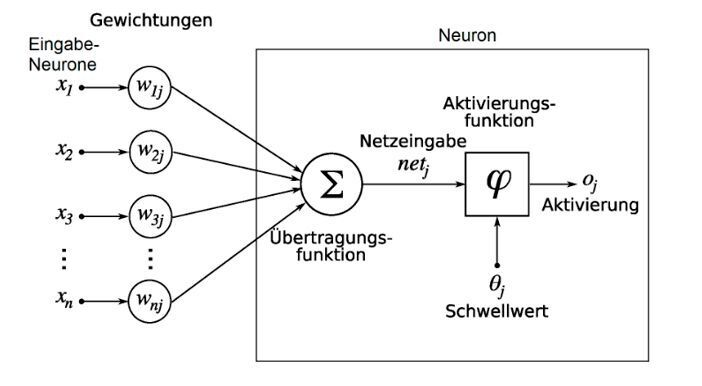
\includegraphics[width=.8\textwidth]{kunstliches_neuron.jpg}
	\caption{Schema eines künstlichen $Neurons_j$ (Quelle: \url{https://www.dev-insider.de/grundbegriffe-und-einfache-beispiele-a-864507/})}
	\label{fig:KünstlichesNeuron}
\end{figure}
Ein künstliches Neuron ist ein mathematisches Modell, das die Funktion eines biologischen Neurons nachahmt. Das künstliche Neuron in Abb. \ref{fig:KünstlichesNeuron} besitzt Eingaben $x_n$, die mit den Dendriten des biologischen Neurons vergleichbar sind. Die Eingabeinformationen können dabei von anderen Neuronen oder aus der Umgebung stammen. \\
Die eingehenden Informationen werden, bevor sie in das Neuron gelangen, mit einer Gewichtung $w_{nj}$ multipliziert. Anschließend werden die Eingaben mithilfe einer Übertragungsfunktion (Propagierungsfunktion) verknüpft, was bedeutet die Werte werden aufsummiert. Das aufsummierte Ergebnis ist die Netzeingabe $net_j$, diese fasst die Informationen zusammen welche in das Neuron gehen. Die Aktivierungsfunktion berechnet die Aktivierung $o_j$, welche je nach Schwellwert $\theta_j$ an alle verbundenen Neuronen weitergeleitet wird. \cite[vgl.][]{JuergenCleve2020}  

\subsubsection{Das Perzeptron}
Ein Perzeptron ist ein einfaches künstliches Neuronales Netz, welches von Frank Rosenblatt als Modell vorgestellt wurde. Als Beispiel wird ein Photo-Perzeptron beschrieben, dass in der Lage ist einfache visuelle Muster zu erkennen. Es besteht aus der Retina (Netzhaut), Assoziationsschicht und der Ausgabeschicht. Die Netzhaut liefert binäre Eingabewerte, welche über gewichtete Verbindungen an die Assoziationsschicht weitergegeben werden. Die Retina Neuronen sind fest mit den Neuronen der Abbildungsschicht verbunden, jedoch sind nicht alle Neuronen miteinander verknüpft. Die Verbindungen zwischen der Abbildungs- und Ausgabeschicht sind hingegen variabel. Während des Trainings, also des Lernens, werden die Gewichtungen  zwischen diesen angepasst. \\
Beim Training werden dem Perzeptron verschiedene Beispiele gezeigt, anhand denen es lernen soll. Ein Beispiel besteht dabei immer aus einem Eingabevektor $x$ und einem Ausgabevektor $y$. Die Aufgabe des Perzeptrons ist es, durch Anpassung der internen Werte zu jedem Eingabevektor $x$, einen passenden Ausgabevektor $y$ zu erzeugen. Das Ziel des Trainings ist es, auf bisher ungesehene, aber ähnliche Eingabevektoren $x'$ ebenfalls einen geeigneten Ausgabevektor $y$ zu assoziieren, in diesem Fall spricht man von einer Generalisierung. \cite[vgl.][]{Scherer1997} \\
Das Perzeptron ist mit seinem Aufbau allerdings beschränkt bei der Klassifikation von Daten. Es ist nur in der Lage linear separierbare Datenmengen zu trennen. Das bedeutet, die Datenmenge kann anhand einer bestimmten Gerade, in zwei separate Datenmengen getrennt werden. Die Ausgaben des Perzeptrons sind also beschränkt auf 0 oder 1, allerdings sind nicht alle Datenmengen trennbar, sondern nur solche deren Trenngerade durch den Ursprung geht.\cite{Ertel2021}

\subsubsection{Aufbau}
Der klassische Aufbau eines Neuronalen Netzes besteht aus einer Eingabeschicht (engl.: Input-Layer), einer oder mehreren versteckten Schichten (engl.: Hidden-Layer), und der Ausgabeschicht (engl.: Output-Layer). Die Eingabeschicht nimmt Werte aus der Umgebung an, und leitet sie weiter an die versteckte Schicht, von wo aus sie an weitere versteckte Schichten oder an die Ausgabeschicht geschickt werden, die das fertige Ergebnis ausgibt. Die Verbindungen der Neuronen zwischen den verschiedenen Schichten besitzen Gewichtungen, mit denen die eingehenden Werte multipliziert werden. Die Komplexität des Aufbaus hängt von der Anzahl der Neuronen und Schichten ab. \cite[vgl.][]{Frochte2020}


\subsubsection{Training eines Neuronalen Netzes}
Das Training eines Neuronalen Netzes ist ein wesentlicher Aspekt des Deep Learnings, bei welchem die Anpassungen der Gewichte und Schwellenwerte innerhalb des Netzwerks stattfinden. Das Training kann oft mehrere Stunden oder sogar Tage dauern, je nach Art und Menge der Daten. Ein Neuronales Netz gilt dann als trainiert, wenn es zu einem Eingabevektor $x$, einen geeigneten Ausgabevekotr $y$ zuverlässig bestimmen kann. Das Netz ist danach in der Lage für bisher ungesehene Eingabevektoren $x'$ ebenfalls passende Ausgabevektoren $y'$ zu zuordnen. \cite[vgl.][]{Scherer1997}

Ein entscheidendes Konzept im Training ist die Fehler- oder Verlustfunktion (engl.: Loss), genauer beschrieben in Abschnitt \ref{subsec:AktivierungsfunktionenVerlust-FunktionenOptimierer}, welche den Unterschied der vorhergesagten Ausgaben mit den tatsächlichen Ergebnissen vergleicht und einen Fehler errechnet. Das Ziel des Trainings ist es, die Verlustfunktion auf ein Minimum zu reduzieren, indem die internen Parameter des Neuronalen Netzes angepasst werden. Die Parameter des Netzwerks werden zu Beginn des Trainings zufällig initialisiert und schrittweise im Training angepasst. \cite[vgl.][]{Choo2020}\\
Die Rückwärtspropagierung (engl.: Backpropagation) ist ein weit verbreitetes Lernverfahren für Neuronale Netze, dass auf eben genannter Minimierung des Fehlers basiert. Für die Rückwärtspropagierung wird im Allgemeinen die Deltalernregel verwendet, die besagt, dass die Fehlerminimierung durch Änderung eines Gewichtes $w_{ij}$ einen Gradientenabstieg bezweckt. Der Ausgangspunkt für diese Lernregel ist wie folgt definiert: 
\begin{equation}
	\Delta_{p}w_{ij} \equiv -\dfrac{dE_p}{dw_{ij}}
\end{equation}
$\Delta_{p}w_{ij}$ entspricht dabei der Änderung eines Gewichts zwischen $i$ und $j$. $dE_p$ ist der gemessene Fehler innerhalb der Lernmenge und $dw_{ij}$ ist die Gewichtung der Neuronen von der Schicht $i$ zur Schicht $j$. \cite[vgl.][]{Rumelhart1986}

Der Backpropagation Algorithmus besteht im wesentlichen aus zwei Schritten, zuerst die Vorwärtspropagierung (engl.: Forwardpropagation) und anschließend die Rückwärtspropagierung.
Der erste Schritt ist die Vorwärtspropagierung, bei dem die Eingabevektoren durch das Netzwerk verarbeitet werden. Die Eingaben werden von Schicht zu Schicht geschickt und durch die Gewichtungen und Aktivierungsfunktionen transformiert. Das Ende dieses Schrittes stellt eine Ausgabe bereit, die dann für den zweiten Schritt weiter verwendet wird. \\
Im nächsten und letzten Schritt des Trainings, der Rückwärtspropagierung, wird die Ausgabe mit dem tatsächlich erwarteten Wert verglichen und anschließend aus der Differenz von Soll- und Ist-Wert ein Fehler errechnet. Als Beispiels Funktion für eine Berechnung eines Fehlers, kann man den mittleren quadratischen Fehler(MSE) verwenden der in \ref{eq:mse} definiert ist.
\begin{equation}
	\label{eq:mse}
	E = \dfrac{1}{2} \sum (Y_i - \hat{Y}_{i})^2
\end{equation}
Nach der Fehlerberechnung, werden die Fehler für die Neuronen der einzelnen Schichten ermittelt. Dabei wird der Beitrag eines jeden Neurons zum Gesamtfehler berechnet. Anschließend wird anhand des Fehlers eines Neurons die Gewichtung von diesem angepasst. Die Gewichte werden dabei mit einem konstanten Faktor $\nu$ und entsprechend des Fehlers mit einem weiteren Term multipliziert. Dieser Prozess wird iterativ wiederholt, bis der Fehler auf ein geeignetes Minimum reduziert wurde. Ist der Fehler auf einen minimalen Wert gesunken und verändert sich nicht mehr großartig, so spricht man davon, dass das \gls{Modell} konvergiert, und das Training beendet werden kann.\cite[vgl.][]{Scherer1997}



\subsection{Aktivierungsfunktionen, Verlust-Funktionen und Optimierer}
\label{subsec:AktivierungsfunktionenVerlust-FunktionenOptimierer}
Für das Training und die allgemeine Funktionalität eines Neuronalen Netzes sind noch einige Komponenten notwendig.\\
Eine Komponente ist die Aktivierungsfunktion, welche bereits in Abschnitt \ref{subsubsec:KünstlichesNeuron} erwähnt wurde. Sie berechnet die Aktivierung $o_j$, welche in Abhängigkeit eines Schwellwertes $\theta_j$ an die nachgelagerten Neuronen weitergegeben wird. Sollte der Schwellwert $\theta_j$ nicht überschritten werden, wartet das Neuron solange auf weitere Eingabesignale und wiederholt die Berechnung der Aktivierung $o_j$, bis der Schwellwert $\theta_j$ überschritten wird und das Neuron seine Ausgabe weitergibt. Es gibt unterschiedliche Aktivierungsfunktionen für verschiedene Zwecke.

Die Identitätsfunktion ist eine einfache Aktivierungsfunktion und sorgt für eine lineare Abbildung der Eingabe auf die Ausgabe. Diese ist für einfache Aufgaben geeignet, wird die Problemstellung komplexer, so eignen sich mehr nicht-lineare Aktivierungsfunktionen wie der Tangens hyperbolicus, \ac{ReLU} oder Sigmoid. Je nach Anwendung und Bedarf wird eine geeignete Funktion ausgewählt. Die Sigmoid-Funktion normalisiert die Ausgaben eines Netzes auf den Bereich zwischen 0 und 1, während der Tangens hyperbolicus einen die Werte in einen Bereich zwischen -1 und 1 bringt. Die \ac{ReLU}-Funktion verhält sich etwas anders zu den vorangegangen Funktionen, da diese für alle positiven Werte die jeweiligen Ausgaben und für alle negativen Werte den Wert 0 zurückgibt. Eine weitere nennenswerte Aktivierungsfunktion ist die Softmax-Funktion, welche ebenfalls Werte in einen Bereich zwischen 0 und 1 überführt, jedoch aber eine Wahrscheinlichkeitsverteilung darstellt. Die Besonderheit der Softmax-Funktion ist die Gegebenheit, dass sich alle Ausgaben zu 1 addieren und somit die Ausgabewerte als Wahrscheinlichkeiten interpretiert werden können.  \cite[vgl.][]{Frick2021} \\
Eine weitere Komponente ist die Verlust-Funktion, welche essenziell für das Trainieren eines Neuronalen Netzes ist. Diese hat zum Ziel, den Fehler, auch Verlust (engl.: Loss) genannt, den ein Netz bei einer Vorhersage produziert, zu minimieren. Ein Fehler entsteht, wenn das Netz eine falsche oder abweichende Ausgabe als erwartet erzeugt. Um den Gesamtfehler eines Netzes zu berechnen, werden die Ausgaben des Neuronalen Netz mit den erwarteten Ergebnissen verglichen. Die Verlust-Funktion hilft dabei den Unterschied zu quantifizieren und den Gesamtfehler des Netzes zu berechnen. \cite{Frick2021}\\
Wie auch bei den Aktivierungsfunktionen gibt es je nach Art der Aufgabe verschiedene Verlust-Funktionen, wie Binary CrossEntropy (BCE), Categorical Cross Entropy, oder Mean Squared Error. Binary Cross Entropy wird verwendet für binäre Klassifikationsprobleme, wie z.B. das Unterscheiden von seriösen und Spam Emails, währenddessen Categorical Cross Entropy für Probleme mit mehr als zwei Klassen verwendet wird. Die Wahl der Verlust-Funktion hängt dementsprechend auch von der Ausgabe des Netzes ab.   

Die letzte wesentliche Komponente ist der Optimierer (engl.: Optimizer), welcher die Gewichte und Biases anpasst, um den Fehler zu minimieren und die Leistung des Netzes zu verbessern. Biases sind zusätzliche Konstanten, die ein Neuron zugeführt bekommt und bei der Berechnung der Ausgabe eine Rolle spielen. Der Bias erhöht die Fähigkeit des Netzes komplexe Beziehungen zwischen Eingaben und Ausgaben zu modellieren und kann so auch nicht-lineare Zusammenhänge erkennen. \\
Es gibt unterschiedliche Arten von Optimierungsalgorithmen, der am häufigsten verbreitete Algorithmus ist der \ac{SGD}, welcher auch Grundlage für weitere Optimierungsverfahren ist. Der \ac{SGD} aktualisiert Gewichte und Biases basierend auf der Ableitung des Verlustes. Dabei wird eine zufällige Stichprobe aus dem Trainingsdatensatz verwendet, um die Berechnung zu beschleunigen. \cite[vgl.][]{Goodfellow2016} \\
Ein anderer Optimierungsalgorithmus ist Adam, der eine Erweiterung des \ac{SGD} ist und eine adaptive Lernrate verwendet, um die internen Parameter des Netze anzupassen. Der Algorithmus erzielt durch die adaptiven Lernraten eine schnellere Konvergenz und eine höhere Genauigkeit als der \ac{SGD}. \cite[vgl.][]{Kingma2014}

\subsection{\acf{CNN}}
\acf{CNN} sind eine spezielle Form von Neuronalen Netzen, die in der Lage sind Bilddaten zu verarbeiten. Sie erkennen mit verschiedenen Filtern Muster, Strukturen und Geometrien in Bildern und können diese anhand dessen klassifizieren. Im nachfolgenden Abschnitt wird der Aufbau und die Funktionsweise eines \ac{CNN}s erklärt, dabei wird auf die verschiedenen Schichten innerhalb des Netzes, sowie auf die mathematische Operation Faltung (engl.: Convolution) eingegangen.

\begin{figure}[ht]
	\centering
	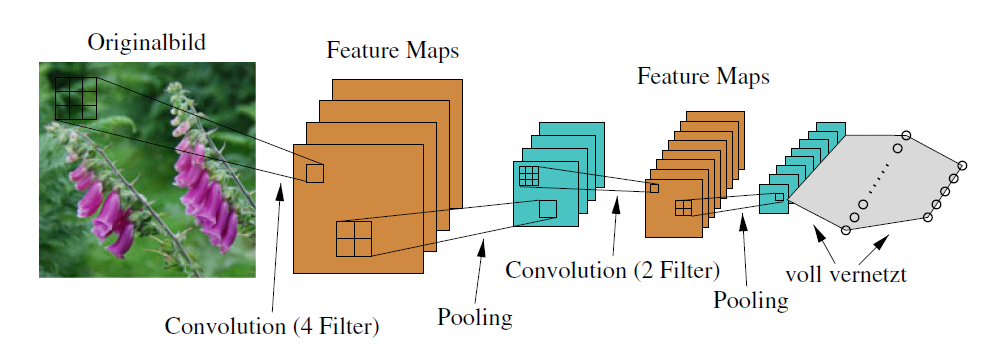
\includegraphics[width=.9\textwidth]{cnn_aufbau.png}
	\caption{Ein \ac{CNN} mit zwei Faltungs-Schichten gefolgt von je einer Pooling-Schicht und am Ende
		zwei voll vernetzten Schichten (Quelle: \cite{Ertel2021})}	
	\label{fig:cnn_aufbau}
\end{figure}

Der Aufbau eines \ac{CNN} besteht aus mehreren Faltungs-Schichten, Pooling-Schichten und voll vernetzten Schichten, wie in Abbildung \ref{fig:cnn_aufbau} zu sehen. 

\paragraph{Convolutional-Layer} ist die Faltungs-Schicht, welche in der Lage ist Merkmale, wie Linien, Kanten und geometrische Formen in Bildern zu erkennen und diese zu extrahieren. Bei einer Faltung wandert ein Filter (engl.: Kernel) über das Eingabebild und erzeugt so ein neues Bild, oder auch sogenannte Feature-Maps. Im mathematischen Sinne gesehen, wandert der Filter über eine Funktion, anstatt über ein Bild und erzeugt somit eine neue. Bei einer Faltung eines Bildes wird meist ein Filter in Form einer 2D-Matrix verwendet, wie er in Gleichung \ref{eq:kernel} als Beispiel zu sehen ist. Die Werte des Filters werden zu Beginn zufällig bestimmt und im Laufe des Trainings angepasst.
\begin{equation}
\begin{bmatrix}
	1 & 2 & 3 \\
	4 & 5 & 6 \\
    7 & 8 & 9
\end{bmatrix}
\label{eq:kernel}
\end{equation}
Der Filter wird schrittweise über das Eingabebild geschoben, wobei jedes Element des Filters mit dem darunterliegendem Bildpunkt des Eingabebildes multipliziert und anschließend aufsummiert wird. Die Summe ist dann das Ergebnis des neuen Bildpunktes. Die Schrittweite des Filters wird als ``Stride'' bezeichnet, und sagt aus, wie viele Bildpunkte, bzw. Pixel, der Filter verschoben wird. Bei einer 2D-Convolution, können zwei Werte für den Stride angegeben werden, die Verschiebung in Richtung der X-Achse und Y-Achse. Die Gleichung \ref{eq:conv_result} zeigt das Ergebnis einer Faltung mit dem Ausdruck aus \ref{eq:conv}.

\begin{equation}
	\begin{pmatrix}
		a_{11} & a_{12} & a_{13} \\
		a_{21} & a_{22} & a_{23} \\
		a_{31} & a_{32} & a_{33}
	\end{pmatrix}
	*
	\begin{pmatrix}
		w_{11} & w_{12} \\
		w_{21} & w_{22}
	\end{pmatrix}
	\label{eq:conv}
\end{equation}

\begin{equation}
	\begin{pmatrix}
		(a_{11}w_{11} + a_{12}w_{12} + a_{21}w_{21} + a_{22}w_{22}) & (a_{12}w_{11} + a_{13}w_{12} + a_{22}w_{21} + a_{23}w_{22}) \\
		(a_{21}w_{11} + a_{22}w_{12} + a_{31}w_{21} + a_{32}w_{22}) & (a_{22}w_{11} + a_{23}w_{12} + a_{32}w_{21} + a_{33}w_{22}) \\
	\end{pmatrix}
	\label{eq:conv_result}
\end{equation}

Es gilt zu beachten, dass das Ergebnis in \ref{eq:conv_result} kleiner ist, als das Ursprungsbild. Dies liegt daran, dass keine Fülldaten (engl.: Padding) verwendet wurde, um die Ränder des Eingabebildes aufzufüllen. Die Größe der Ergebnismatrix lässt sich durch Gleichung \ref{eq:conv_size} berechnen, wobei $W$ die Eingabegröße des Bildes, $F$ die Filtergröße, $S$ der Stride und $P$ das Padding ist. \cite[vgl.][]{Teoh2023}

\begin{equation}
	W_{out}= \dfrac{W+2P-F}{S}+1
	\label{eq:conv_size}
\end{equation}

\paragraph{Pooling-Layer} dient zur Extraktion von Merkmalen (engl.: Features) des Bildes, welche eine hohe semantische Bedeutung haben. Die Eingaben dieser Schicht, sind die Ausgaben der vorangegangenen Faltungs-Schicht. Diese Schicht verwendet entweder das Maximal- oder Mittelwert-Pooling (engl.: Max- oder Average-Pooling). Dabei werden überflüssige und redundante Informationen aus der Datenmenge entfernt. Durch das Entfernen der unwesentlicher Bestandteile reduziert sich Berechnungszeit und die Merkmale werden verdichtet. 

Beim Pooling wandert ebenfalls ein Filter, meist mit einer Größe von $2x2$, und einer Schrittweite von zwei über das Bild. In Abbildung \ref{fig:pooling} werden die zwei Arten des Poolings durchgeführt. Das Max-Pooling extrahiert jeweils den höchsten Wert welcher innerhalb der Filter-Matrix liegt. Das Average-Pooling nimmt jeweils den Mittelwert aller Elemente innerhalb der Filter-Matrix. Durch das Pooling verkleinert sich das Bild je nach Filtergröße und Schrittweite.\cite[vgl.][]{Teoh2023} Im Beispiel von Abbildung \ref{fig:pooling} verkleinert sich das Ausgangsbild um die Hälfte, die Größe nach dem Pooling berechnet sich ebenfalls mit der Formel aus \ref{eq:conv_size}.

\paragraph{Fully-Connected-Layer} oder auch voll verknüpfte Schicht, bildet den Abschluss eines \ac{CNN}s. Die Merkmale der vorangegangenen Schicht, also des Pooling-Layers, werden hier mit allen Ausgabemerkmalen verknüpft, es handelt sich dabei um ein normales Neuronales Netz. 

Zunächst muss aus der Ausgabe der vorangegangenen Schicht eine 1D-Matrix erstellt werden, diesen Prozess nennt man auch ``flatten''. Zuletzt wird schließlich jedes Element aus der 1D-Matrix, mit jedem Element der Ausgabe-Schicht verbunden. Die Ausgabe des Netzes zeigt dann z.B. die Klassifikation eines Bildes, in dem berechnet wird, welches Ausgabeelement die höchste Wahrscheinlichkeit besitzt. \cite[vgl.][]{Weidman2020}

\begin{figure}
	\centering
	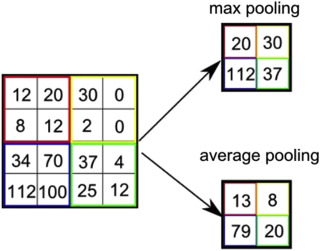
\includegraphics[width=.6\textwidth]{pooling.jpg}
	\caption{Maximal und Mittelwert-Pooling, sowie das Ergebnis der beiden Methoden. (Quelle: \url{https://www.sciencedirect.com/topics/mathematics/pooling-layer})}
	\label{fig:pooling}
\end{figure}


\subsection{Over- und Underfitting}
Over- und Underfitting sind zwei Probleme, die beim Training eines Neuronalen Netzes auftreten können. Diese Probleme beeinflussen die Generalisierungsfähigkeit des Modells, also die Fähigkeit auf neuen und bisher ungesehene Daten gute Ergebnisse zu erzielen.\\
Overfitting tritt auf, wenn sich ein Modell zu stark auf die Trainingsdaten abgestimmt hat und somit keine generelle Strukturen mehr erkennt. Das \gls{Modell} hat sich in diesem Fall die Trainingsdaten gemerkt und kann daher nur schlecht gute Ergebnisse auf neuen Daten erzielen. Ist die Kapazität des \gls{Modell}s zu groß, so neigt das Neuronale Netz dazu kleine Schwankungen in den Daten zu lernen und verliert somit die Generalisierung der Daten.\\
Beim Underfitting hingegen, ist das \gls{Modell} nicht in der Lage eine zugrundeliegende Struktur innerhalb der Daten zu erkennen, was zu einer schlechten Leistung bei den Trainings- und auch bei den Testdaten führt. Im Falle des Underfittings hat das \gls{Modell} meist eine zu geringe Kapazität, um sich alle relevanten Informationen zu speichern.\cite[vgl.][]{Goodfellow2016}
%!TEX root = ../../main.tex
\section{Magnetresonanztomographie (MRT)}
Die \ac{MRT}, auch Kernspintomographie genannt, ist ein bildgebendes Verfahren zur Darstellung von Struktur und Funktion der Weichteile und Organe im Körper. Mit einer \ac{MRT} können Schnittbilder des Körpers oder einzelner Körperteile erstellt werden. Für die Bildgebung werden starke Magnetfelder verwendet, diese sind jedoch unbedenklich für den menschlichen Körper, da bei diesem Verfahren keine \gls{Ionisierende Strahlung} verwendet wird. \cite[vgl.][]{Kramme2016}\\
\begin{figure}[ht]
	\centering
	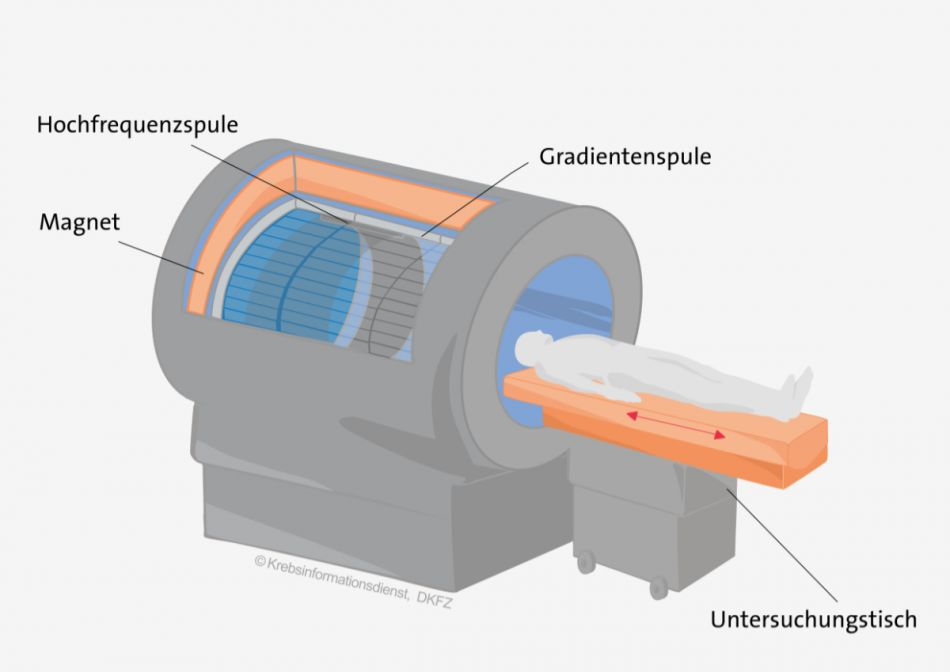
\includegraphics[width=.9\textwidth]{mrt_aufbau.jpg}
	\caption{Schematischer Aufbau eines Magnetresonanztomographen (Quelle: \url{https://www.krebsinformationsdienst.de/untersuchung/bildgebung/kernspintomographie.php})}
\end{figure}

Der Magnetresonanztomograph besteht aus mehreren Komponenten: 
\begin{itemize}
	\item einem supraleitenden Hauptmagneten in einer Röhre, der ein starkes und konstanten Magnetfeld erzeugt. Ein supraleitender Magnet wird durch flüssigen Stickstoff gekühlt, sodass der Spulenwiderstand nahezu null wird. Dies ermöglicht die Erzeugung starker Magnetfelder.
	\item einem Gradientensystem, das zusätzliche Magnetfelder generiert, die je nach Position im Körper unterschiedlich sind und so eine räumliche Auflösung ermöglichen.
	\item einem Hochfrequenzsystem, welches aus einem Sende- und Empfangsspulensystem besteht. Dieses sendet Radiowellen zur Anregung der Wasserstoffatome aus, welche dadurch ihrer Ausrichtung verlieren.
	\item einem Computersystem, das geeignet ist für die Verarbeitung der Daten eines \ac{MRT}s
	\item und einem Untersuchungstisch, auf welchem der Patient während der Untersuchung liegt
\end{itemize}
Das Verfahren basiert auf einem physikalischen Prinzip, dem Eigendrehimpuls auch Spin genannt. Dabei dreht sich ein \gls{Proton} um seinen eignen Schwerpunkt (Kernspin) und erzeugt durch die Rotation ein Magnetfeld. Die Wasserstoffkerne in unserem Körper besitzen ebenfalls einen Spin und verhalten sich so wie kleine Magnete, die ein messbares Magnetfeld erzeugen.\\
Die Kernspins sind im Normalzustand ungeordnet, legt man jedoch ein starkes Magnetfeld an, so richten sich die Kernspin-Achsen entlang den magnetischen Feldlinien aus. Sie führen dabei eine Kreiselbewegung aus, bei der sie sich immer näher an die Feldlinien bewegen, aber sich niemals ganz daran ausrichten, dies wird auch als Präzessionsbewegung bezeichnet. Die Frequenz dieser Bewegung nennt sich die Larmorfrequenz.\\ 
Allein durch die Ausrichtung der Kernspins erfolgt noch keine Bildgebung, es muss zunächst ein hochfrequenter Impuls (HF-Impuls) senkrecht zum Hauptmagnetfeld gegeben werden. Der Impuls muss dabei eine bestimmte Frequenz besitzen, nämlich die der Kernspins, also die Larmorfrequenz. Durch diesen Impuls synchronisieren sich die Protonen und manche der Kernspin-Achsen kippen um 90°, wobei sie bei diesem Vorgang Energie aufnehmen.\cite[vgl.][]{ChristophPabst2013}\\
Nach dem Impuls, kippen die Kernspins wieder zurück in ihre ursprüngliche Lage entlang des Hauptmagnetfeldes. Beim Ausrichten in die ursprüngliche Position, wird die aufgenommene Energie in Form von wärme wieder an die Umgebung abgegeben. Dieser Prozess der Wiederausrichtung wird als longitudinale Relaxation oder ``T1-Relaxation'' bezeichnet. Hierbei kommt es auf die Wärmeleitfähigkeit des Gewebes an. Ein weiterer Prozess der beim Ausschalten des HF-Impulses in Gang gesetzt wird, ist der Verlust der synchronen Kreiselbewegung, wodurch die transversal Magnetisierung verloren geht. Unterschiedliche Gewebe können die transversal Magnetisierung unterschiedlich lang aufrecht erhalten und erzeugen so Kontraste auf den Bildern, dies wird auch als ``T2-Relaxation'' bezeichnet. Man misst im wesentlichen die Dauer der verschiedenen Prozesse und kann anhand dessen auf die Gewebearten schließen und daraus die Kontraste berechnen.\cite[vgl.][]{Kernspin2022}

Es können zusätzlich Kontrastmittel verwendet werden, um bestimmte Teile heller erscheinen zulassen. Je nach Art des Kontrastmittels werden andere Bereicher dunkler, bzw. heller dargestellt. Die Kontrastmittel selbst sind nicht auf dem Bild zusehen, jedoch ihre Auswirkungen auf das umliegende Gewebe, so erscheint bei einer kontrastverstärkten T1-Gewichtung die Umgebung wie z.B. Blut oder Tumore heller. \cite[vgl.][]{ChristophPabst2013}

Es gibt weitere Methoden für eine \ac{MRT}, um bestimmte Strukturen, Gewebearten oder Flüssigkeiten heller bzw. dunkler erscheinen zu lassen. Eine davon ist die Flair-Gewichtung (fluid-attenuated inversion recovery), eine spezielle Methode zur Unterdrückung von Flüssigkeiten auf den entstehenden Bildern. Es unterdrückt z.B. das Liquor im Gehirn, wodurch bestimme Tumore besser sichtbar werden. Besitzt der Tumor jedoch einen hohen Wasseranteil, so wird dieser ebenfalls auf dem Bild unterdrückt. \cite[vgl.][]{Gizewski2001}
%%!TEX root = ../../main.tex
\chapter{PyTorch}
\section{Einführung}
PyTorch ist ein Open-Source Bibliothek für Python, die von Facebook entwickelt wurde. Die Bibliothek ist speziell für Maschinelles Lernen und Künstliche Intelligenz ausgelegt und bietet eine große Anzahl von Tools und Funktionen für das Entwickeln von Deep Learning-Modellen. Es ist dafür bekannt mit dynamischen Berechnungsgraphen zu arbeiten, welche für das Entwickeln von Prototypen geeignet sind, da Änderungen zur Laufzeit vorgenommen werden können. PyTorch besteht aus mehreren Hauptkomponenten und bietet ein vielfältiges Ökosystem, das je nach Bedarf verwendet werden kann. Es gibt unter anderem ``torchvision``, das für die Verarbeitung von visuellen Daten geeignet ist, ``torchaudio`` für die Verarbeitung von Audiodateien und noch weitere Komponenten. Das Ökosystem besteht aus vielen zusätzlichen Möglichkeiten noch schneller und einfacher zu arbeiten. Alle Funktionen, die für das Maschinelle Lernen benötigt werden, sind direkt ab Installation mit angeboten und können verwendet werden. Tensoren sind die Hauptdatenstrukturen für alle Berechnungen und sind eine Art multidimensionale Matrizen, genaueres dazu in Abschnitt \ref{sec:Tensoren}. PyTorch bietet die Möglichkeit alle Rechenoperationen auf der \acs{GPU}, also dem Grafikprozessor, auszuführen, um so schnellere Berechnungen durchzuführen. \cite[vgl.][]{PyTorch}

\section{Tensoren}
\label{sec:Tensoren}
Ein Tensor ist eine Datenstruktur die in PyTorch verwendet wird, um Daten zu speichern oder verändern. Diese sind multidimensionale Arrays, zu deutsch Listen, die verschiedene Strukturen, wie Skalare,Vektoren, Matrizen und Tensoren darstellen können. \\

\paragraph*{Skalar} ist eine einfache Zahl, wie z.B. eine 1.
\paragraph*{Vektor} ist ein ein-dimensionaler Array \begin{small}$\left(\begin{array}{c} 1 \\ 0 \\ 1 \end{array}\right)$\end{small}
\paragraph*{Matrix} ist ein zwei-dimensionaler Array $\begin{bmatrix}
	1 & 2 \\
	4 & 3  
\end{bmatrix}$.
\paragraph*{Tensor} ist $n$-dimensionaler Array $\begin{pmatrix}
 \begin{bmatrix} 1 & 2 \\	3 & 4  \end{bmatrix} &  \begin{bmatrix} 9 & 10 \\ 11 & 12  \end{bmatrix}\\
\begin{bmatrix}	5 & 6 \\	7 & 8  \end{bmatrix} &  \begin{bmatrix} 13 & 14 \\ 15 & 16  \end{bmatrix}
\end{pmatrix}$

Tensoren können verwendet werden um verschiedene Rechenoperationen wie addieren, subtrahieren, multiplizieren oder dividieren durchzuführen. Darüber hinaus bietet ein Tensor noch mehr Funktionen wie das Konvertieren von einer Ganzzahl in eine Fließkommazahl, oder auch Funktionen um den Maximalwert in einem Tensor zu bekommen. \\
Ein Vorteil von Tensoren ist die Fähigkeit die Operationen auf der \ac{GPU} ausführen zu lassen. \cite[vgl.][]{PapaJoe}



\section{CUDA}

%!TEX root = ../../main.tex
\chapter{Material und Methoden}
\section{Datensatz: \ac{BraTS}}
Der \ac{BraTS} Datensatz ist ein öffentlich verfügbarer Datensatz, der für die Entwicklung und Evaluierung von \glspl{Modell} für die Segmentierung von Gehirntumoren verwendet wird. Er wurde von der Radiological Society of North America in Partnerschaft mit der American Society of Neuroradiology(ASNR) und Medical Image Computing and Computer Assisted Interventions(MICCAI) erstellt und besteht aus über tausend \ac{MRT} Bildern von verschiedenen Patienten mit Hirntumoren. \cite[vgl.][]{RSNABrainTumor2021}

\subsection{Beschreibung}
\label{subsec:Beschreibung}
Der Datensatz enthält multi-institutionellen und multi-parametrischen \ac{MRT} Scans (mpMRT), die unter klinischen Standardbedingungen mit unterschiedlichen Geräten und Protokollen aufgenommen wurden. ``Multi-institutionell'', bezieht sich darauf, dass die Daten für den Datensatz von mehreren medizinischen Einrichtungen bereitgestellt und zusammengeführt wurden. ``Multi-parametrisch'' bedeutet, dass der Datensatz mehrere Parameter bzw. Merkmale enthält, welche für die Segmentierung der Hirntumore verwendet werden können. \\
Für die Aufgabe der Segmentierung wurden alle Gehirntumore mit den führenden BraTS-Algorithmen segmentiert und anschließend von freiwilligen Neuroradiologie Experten mit unterschiedlicher Erfahrung nochmals verfeinert. Für die manuellen Beschriftung der Daten wurde ein strenges Protokoll eingehalten, um einheitliche Daten zu erhalten. Abschließend wurden die manuell verfeinerten Bilder von zertifizierten und erfahrenen Neuro-Radiologen mit mehr als 15 Jahren Erfahrung in dieser Tätigkeit bestätigt. 
Die beschrifteten Tumor-Regionen basieren auf den VASARI-Merkmalen\footnote{VASARI-Merkmale(Visually Accesable Rembrandt Images) sind ein System für die konsistente Beschreibung von Gliomen (Tumoren) mithilfe definierter visueller Merkmale \cite[vgl.][]{Nam2021}}, welche für einen geschulten Radiologen sichtbar sind. Diese Merkmale umfassen den mit Gadolinium anreichernden Tumor (Kennzeichnung 4), das peritumorale ödematöse/invasive Gewebe (Kennzeichnung 2) und den nekrotischen Tumorkern (Kennzeichnung 1). \cite[vgl.][]{Baid2021}
\begin{figure}[ht]
	\centering
	\begin{subfigure}[b]{0.4\textwidth}
		\centering
		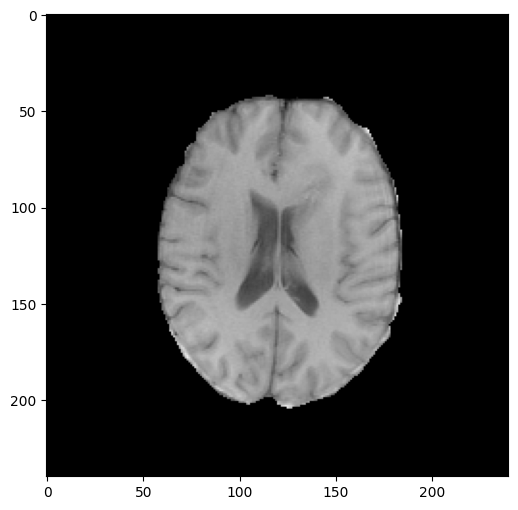
\includegraphics[width=\linewidth]{mrt_t1.png}
		\caption{T1-Gewichtung}
		\label{fig:t1}
	\end{subfigure}
	\hfill
	\begin{subfigure}[b]{0.4\textwidth}
		\centering
		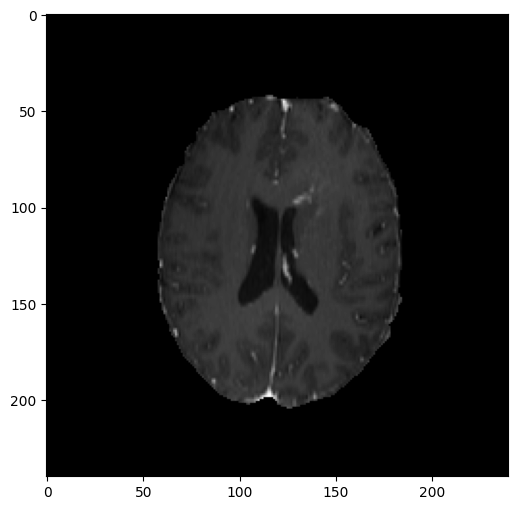
\includegraphics[width=\linewidth]{mrt_t1ce.png}
		\caption{kontrastverstärkte T1-Gewichtung}
		\label{fig:t1ce}
	\end{subfigure}
	\vskip\baselineskip
	\begin{subfigure}[b]{0.4\textwidth}
		\centering
		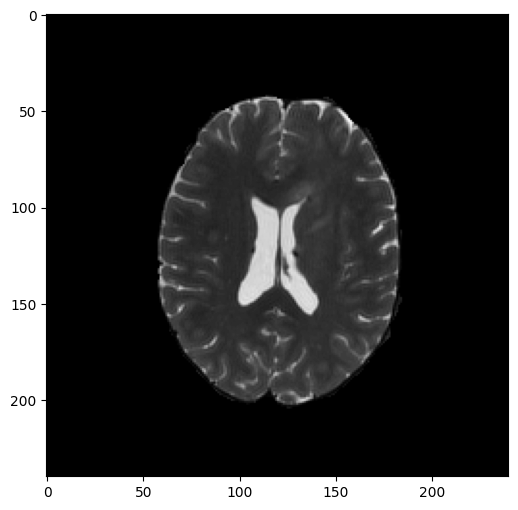
\includegraphics[width=\linewidth]{mrt_t2.png}
		\caption{T2-Gewichtung}
		\label{fig:t2}
	\end{subfigure}
	\hfill
	\begin{subfigure}[b]{0.4\textwidth}
		\centering
		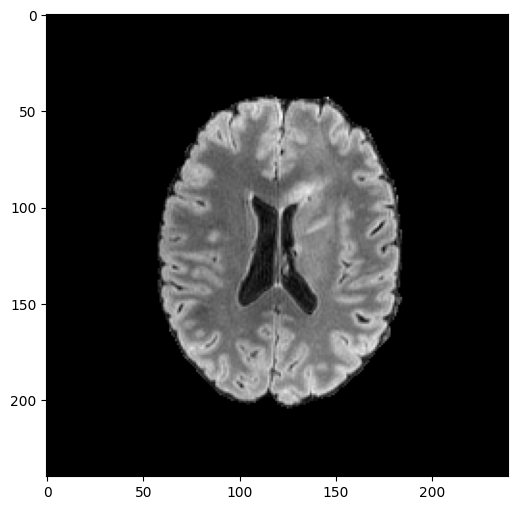
\includegraphics[width=\linewidth]{mrt_flair.png}
		\caption{Flair-Gewichtung}
		\label{fig:flair}
	\end{subfigure}
	\caption{Die vier Modalitäten im Datensatz}
	\label{fig:mrt_scans}
\end{figure} 

Der Datensatz enthält 1251 Einträgen, jeder Eintrag besteht aus einer T1-, kontrastverstärkte T1-, T2- und Flair-Gewichtung (siehe Abb. \ref{fig:mrt_scans}) sowie einer fertigen Segmentierung des Hirntumors. Die Dateien selbst sind im NIfTI-Dateiformat, was für ''Neuroimaging Informatics Technology Initiative`` steht und ein gängiges Format für medizinische Bilddaten ist. Das Dateiformat enthält die 3D-Volumendaten, welche aus mehreren Schichten von Bildern bestehen. Jedes Voxel, ein 3D-Bildpunkt, enthält einen numerischen Wert, der das Signal bzw. den Kontrast widerspiegelt. Zusätzlich enthält das NIfTI-Dateiformat Metadaten, wie die räumliche Orientierung, Bildgröße,Raumkoordinaten und weitere Metadaten. \cite[][]{NIfTI} Die Bilder liegen in einer Größe von 150x240x240 Pixeln vor, dies entspricht wie bereits erwähnt den 3D-Volumendaten, welche in 150 Schichten aufgeteilt wurden, wobei jede Schicht ein Bild in der Größe von 240x240 Pixeln entspricht.


\subsection{Vorverarbeitung}
Die Vorverarbeitung der Daten ist ein wichtiger Schritt, damit sich die Qualität und Effektivität des Trainings von einem Neuronalen Netz verbessern. Der bereitgestellte Datensatz wurde bereits einer Standard Vorverarbeitung (engl.: Pre-Processing) unterzogen. Zunächst wurden die Daten vom DICOM-Dateiformat in das NIfTI-Dateiformat konvertiert, was zur einfacheren Handhabung der Daten dient. Ebenfalls wurde eine Anpassung auf gleiche anatomische Vorlage und isotrope Auflösung getätigt. Abschließend wurde  das Skull-Stripping\footnote{Skull-Stripping ist der Prozess des Entfernens von Schädel und anderen nicht auf das Hirn bezogenen Strukturen vom Bild. \cite[vgl.][]{SwiebockaWiek2016}} durchgeführt um irrelevante Strukturen zu entfernen. \cite[vgl.][]{Baid2021}

\paragraph{Normalisierung}
Nach diesen Schritten sind die Daten noch nicht für das Training eines Neuronalen Netzes geeignet. Die Daten müssen zunächst normalisiert werden, dies kann auf zwei Wegen geschehen. Entweder die Werte werden auf einen Bereich von 0 bis 1 skaliert oder man verwendet die Z-Standardisierung. Bei einer einfachen Skalierung der Werte wird folgende Gleichung verwendet
\begin{equation}
	f(x)=\frac{x - min(x)}{max(x) - min(x)}
\end{equation}

Dies führt zwar zu einer Vereinheitlichung der Werte, jedoch ist die Verteilung der Merkmale im Bild so nicht normiert. Für dieses Vorhaben verwendet man die Z-Standardisierung, welche den Mittelwert der Daten auf 0 und die Standardabweichung auf 1 bringt. Es wird verhindert, dass bestimmte Merkmale dominant werden, im Vergleich zu anderen. Zudem wird die Genauigkeit des \glspl{Modell} erhöht.\cite[vgl.][]{Goodfellow2016} Die gleich für die Z-Standardisierung lautet
\begin{equation}
	f(x)=\frac{x - \mu_x}{\sigma_x}
\end{equation}
wobei $\mu_x$ der Mittelwert und $\sigma_x$ die Standardabweichung des Datensatzes ist. Diese Werte müssen vorab berechnet werden, in dem der Mittelwert und die Standardabweichung von jedem Bild berechnet wird, anschließend aufsummiert und durch die Anzahl der Bilder geteilt wird
\begin{equation}
	\begin{aligned}
		\mu &= \frac{1}{n}\sum_{i=1}^{n}x_i \\ \\
		\sigma &= \sqrt{\frac{1}{n}\sum_{i=1}^{n}(x_i - \mu)^2}
	\end{aligned}
\end{equation}
wobei $n$ die Anzahl der Bilder und $x_i$ ein Bild des Datensatzes ist.

\paragraph{Data Augmentation} 
Im medizinischen Bereich sind die Bilddaten oft begrenzt, weshalb sich das Training eines Neuronalen Netzes dadurch erschwert. Eine Methode dem entgegen zu wirken ist die Data Augmentation, bei welcher die Diversität des Trainingsdatensatzes erhöht wird. Verschiedene Augmentierungen sind Bildbearbeitungsmethoden wie das Rotieren, Skalieren, Ausschneiden oder auch Spiegeln eines Bildes. Es ist wichtig darauf zu achten, dass alle Augmentierungen sowohl auf die Eingangsbilder, als auch auf die dazugehörigen Segmentierungen angewendet werden, da das Neuronale Netz sonst falsche Masken für die Eingaben erlernt. \cite[vgl.][]{Shorten2019}

\paragraph{3D-Bild zu 2D-Bilder} 
Die Daten liegen als 3D-Bilddaten vor, jedoch ist die Anzahl der Daten mit 1251 Bildern eher gering. Um mehr Bilder aus den vorhandenen Daten zu bekommen, werden die 3D-Bilder in einzelne 2D-Bilder geschnitten. Wie bereits in Abschnitt \ref{subsec:Beschreibung} erwähnt, besteht ein 3D-Bild aus 150 geschichteten Bildern mit der Größe von 240x240 Pixeln. Jede einzelne Schicht wird als Separates Bild abgespeichert, um so die Anzahl der Daten zu erhöhen, so entstehen aus einem 3D-Bild 150 einzelne 2D-Bilder. Es wird jedoch nicht nur die Anzahl der Daten erhöht, sondern auch die Geschwindigkeit der Berechnungen, da dies im zweidimensionale weniger Rechenleistung und Speicher benötigt. Die Konvertierung von 3D- in 2D-Bilder bringt aber auch Nachteile mit sich, wie der Verlust des räumlichen Zusammenhangs zwischen den einzelnen Schichten. \cite[vgl.][]{Stevens2020}

\paragraph{Größen Skalierung}
\label{paragraph:GrößenSkalierung}
Bei manchen Neuronalen Netzen, kann die Größe des Bildes eine Rolle spielen. Es gibt Architekturen, bei denen die Bildgröße beliebig sein kann, oder das Eingabebild eine bestimmte Größe vorweisen muss, damit es verarbeitet werden kann. \\
Die Architektur welche für die Segmentierung der Gehirntumore verwendet wird, ist ein U-Net und wird in Kapitel \ref{sec:Modellarchitektur} genauer beschrieben. Aufgrund der besonderen Architektur des UNets, müssen die Bilder eine bestimmte Größe haben. Der Grund für die spezifische Eingabegröße liegt in der Architektur des UNets, genauer gesagt durch die Down- und Upsampling Pfade. Die Größe des Bildes, wird schrittweise durch Konvolution und Max-Pooling Schichten auf der einen Seite reduziert und auf der anderen Seite wieder vergrößert. \\
Aufgrund des Designs des U-Net muss die Größe der Bilder ein Vielfaches von der Anzahl der Downsampling-Schichten sein. Die Größe der Bilder wird durch die Gegebenheiten definiert durch $2^N$, wobei $N$ die Anzahl der Downsampling-Schichten ist. Sei $N=4$, so muss die Eingabegröße der Bilder ein vielfaches von $2^4=16$ sein. Ist nicht die richtige Größe gegeben, so kann es zur Inkonsistenz der Größen kommen, was wiederum die Leistung des \gls{Modell}s beeinflusst. \cite[vgl.][]{Ronneberger2015}

Um die Bilder in eine geeignete Größe zu bringen werden sie von der Mitte ausgehend nach außen hin ausgeschnitten. Die Größe des Bildausschnittes beträgt im Grunde 128x128 Pixel. Es kommt jedoch vor, dass Teile des Gehirns abgeschnitten werden (siehe Abb. \ref{fig:GrößeOhnePuffer}), weshalb noch ein Puffer von 60 Pixeln je Rand hinzugefügt wurde. Nach Hinzufügen des Puffers ist das Bild nicht mehr in einer geeigneten Größe und wird abschließend auf eine Größe von 128x128 Pixeln skaliert (siehe Abb. \ref{fig:GrößePuffer}).
\begin{figure}[ht]
	\centering
	\begin{subfigure}[b]{0.4\textwidth}
		\centering
		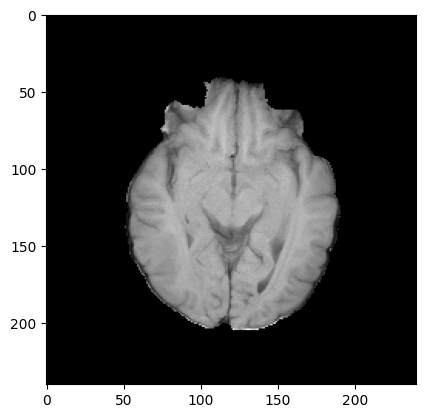
\includegraphics[width=\linewidth]{img_size_original.png}
		\caption{Original Bild}
		\label{fig:GrößeOrg}
	\end{subfigure}
\vfil
	\begin{subfigure}[b]{0.4\linewidth}
		\centering
		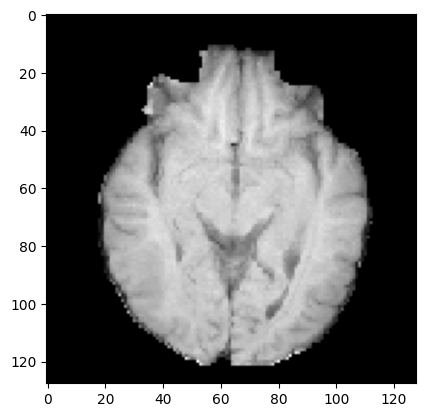
\includegraphics[width=\textwidth]{img_size_crop_puffer.png}
		\caption{Ausschnitt mit Puffer}
		\label{fig:GrößePuffer}
	\end{subfigure}
\hfil
	\begin{subfigure}[b]{0.4\linewidth}
		\centering
		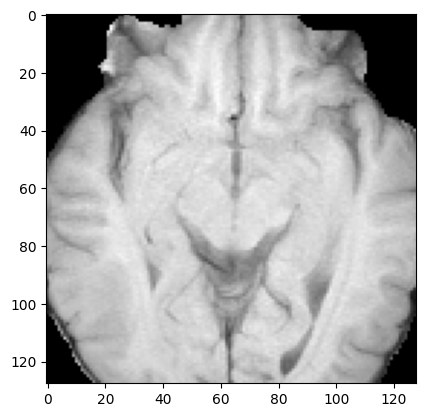
\includegraphics[width=\textwidth]{img_size_crop.png}
		\caption{Ausschnitt ohne Puffer}
		\label{fig:GrößeOhnePuffer}
	\end{subfigure}
	\caption{Orginal Bild (T1-Gewichtung) im Vergleich zum Ausschnitt mit und ohne Puffer.}
\end{figure} 


\subsection{Aufteilung}
Es ist wichtig den Datensatz in verschiedene Teile aufzuteilen, damit die Entwicklung eines Modells gelingt. Der Datensatz wird dafür in einen Trainings-, Validerungs- und Testdatensatz aufgeteilt. Diese verschiedenen Datensätze ermöglichen es die Leistung und die Generalisierungsfähigkeit des \gls{Modell}s zu beurteilen. \\
Der Trainingsdatensatz wird verwendet, um das Modell zu trainieren, indem es die internen Modellparameter anhand der Eingabedaten und den dazugehörigen Beschriftungen anpasst. Je größer der Trainingsdatensatz ist, desto besser kann das \gls{Modell} generalisieren, da es viele Daten mit unterschiedlichen Merkmalen lernt. \\
Um die Leistung des \gls{Modell}s während des Trainings zu beurteilen wird der Validierungsdatensatz verwendet. Anhand der Ergebnisse auf dem Validierungsdatensatz, werden die Hyperparameter des \gls{Modell}s angepasst. Es ist wichtig darauf zu achten, dass dieser Datensatz keine Überschneidungen mit dem Trainingsdatensatz hat, da es sonst zu falschen Ergebnissen kommt. \cite[vgl.][]{Weidman2020}
Möchte man das Modell abschließend nochmals evaluieren, so kommt oft ein Testdatensatz zum Einsatz, den das \gls{Modell} noch nie vorher gesehen hat. Nach dem das Training mit dem Trainings- und Validierungsdatensatz abgeschlossen ist, kann der Testdatensatz herangezogen werden, um die finale Leistung des \glspl{Modell} zu beurteilen.
%!TEX root = ../../main.tex
\section{Modellentwicklung}
Die Entwicklung des \gls{Modell}s ist ein anspruchsvolles Unterfangen, welches im nachfolgenden Kapitel genauer erläutert wird. Zunächst wird die Architektur des \gls{Modell}s vorgestellt und wie dieses aufgebaut ist. Der nächste Punkt erklärt was Hyperparameter sind und was diese bewirken, gefolgt von den Problemen bei der Entwicklung, sowie die Implementierung mit PyTorch. Zum Schluss wird noch der Prozess des Trainings beschrieben.
\subsection{Architektur des Neuronalen Netzes}
\label{sec:Modellarchitektur}
Die gewählte Architektur ist ein U-Net, das seinen Namen aufgrund seines U-förmigen Aufbaus (siehe Abb. \ref{fig:unet_aufbau}) bekommen hat. Das U-Net wurde speziell für die Segmentierung biomedizinischer Bilder entwickelt und ist eine spezielle Form von \ac{CNN}s. Das U-Net ist speziell darauf ausgelegt auch mit kleinen Datensätzen gute Ergebnisse zu erzielen. In der Medizin stehen oft nur begrenzt beschriftete Daten zur Verfügung, da der Aufwand für die Beschriftung der Daten hoch ist. Aufgrund dieser Tatsache ist das U-Net für diese Zwecke besonders geeignet. Die folgende Beschreibung der Architektur basiert auf dem originalen U-Net und wird in dieser Arbeit als Basis für das \gls{Modell} verwendet, welches genauer in Abschnitt \ref{subsec:Implementierung} beschrieben wird.

\begin{figure}
	\centering
	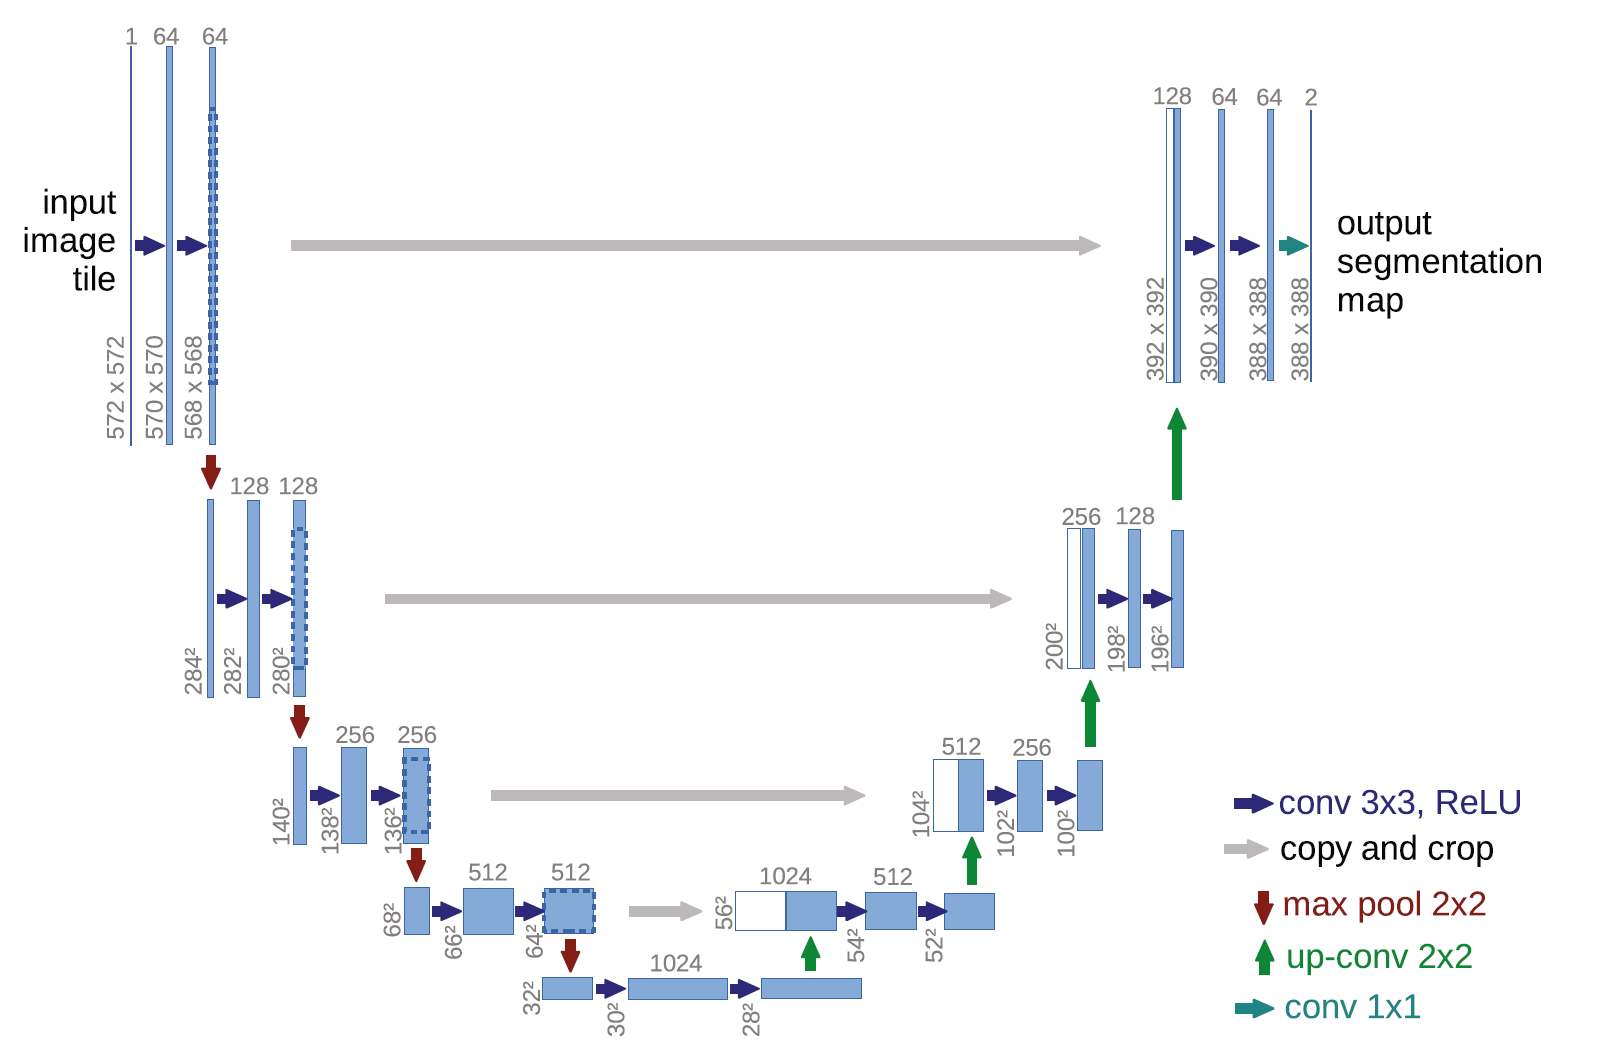
\includegraphics[width=.9\textwidth]{unet_aufbau.png}
	\caption{Aufbau eines U-Nets mit einem Encoder und Decoder Abschnitt für die Extrahierung von Merkmalen und die Wiederherstellung des Original Bildes mit der fertigen Segmentierung (Quelle: \cite{Ronneberger2015})}
	\label{fig:unet_aufbau}
\end{figure}
Die Architektur des Netzes besteht aus zwei Teilen, dem Downsampling Pfad, auch Encoder genannt, und dem Upsampling Pfad, der Decoder. Der Encoder ähnelt einem klassischen \ac{CNN} und besteht aus einer reihe von Convolutional und Max-Pooling Operationen, wobei es jedoch keine vollständig vernetzen Schichten gibt. 

Der Encoder wird verwenden, um die Feature-Maps aus dem Bild zu extrahieren. Bei jedem Schritt, den die Eingabe durch den Encoder macht, werden mehr Feature-Maps extrahiert und die räumliche Dimension des Bildes verringert. Die Ausgabe wird an die nächsthöhere Schicht weitergegeben, dies dient dazu möglichst viele Details auf verschiedenen Ebenen zu erhalten. Der Aufbau besteht dabei aus einer Reihe von zweifach Faltungen mit einem 3x3 Filter, auf die jeweils immer eine Max-Pooling Schicht mit einer Filtergröße von 2x2 und einer Schrittweite von 2 folgt. Bei jedem Encoder Schritt wird die Anzahl der Filter, bzw. Feature-Maps in den Faltungsschichten verdoppelt.

Im Decoder wird die komprimierte Eingabe wieder auf die ursprüngliche Bildgröße skaliert, auch ''Upsampling`` genannt. Dies geschieht durch eine Aneinanderreihung von Upsampling Schichten jeweils gefolgt von zweifach Faltungen und einer Aktivierungsfunktion. Nach jedem Upsampling der Feature-Maps folgt eine Faltung mit einem 2x2 Filter, welche die Anzahl der Feature-Maps jeweils halbiert. Hierbei findet zusätzlich eine Verkettung der Feature-Maps aus dem entsprechenden Encoder Abschnitt statt. Nach der 2x2-Faltung folgen jeweils immer zwei 3x3-Faltungen mit einer abschließenden ReLU Aktivierungsfunktion. Abschließend an den Decoder Abschnitt folgt noch eine Faltung mit einem 1x1 Filter, der die Features auf die gewünschte Anzahl von Klassen der Segmentierungsaufgabe abbildet. \cite[vgl.][]{Ronneberger2015}

\subsection{Hyperparameter}
Hyperparameter sind Parameter, deren Werte vor dem Training eines \gls{Modell}s festgelegt und während des Trainings, bis auf gewisse Ausnahmen nicht angepasst werden. Sie sind entscheidend für die Leistung des Modells und müssen sorgfältig ausgewählt werden. Die Auswahl der richtigen Hyperparameter ist oft eine Kunst und erfordert sowohl Erfahrung als auch experimentelles Ausprobieren. 

In der Praxis wird häufig eine Technik namens Hyperparametersuche oder -optimierung verwendet, bei der verschiedene Kombinationen von Hyperparametern systematisch ausprobiert werden, um diejenige zu finden, die die beste Leistung liefert. In diesem Abschnitt werden die wichtigsten Hyperparameter, die bei der Entwicklung des eines Deep Learning \glspl{Modell} relevant sind genauer beschrieben.

\paragraph{Lernrate} Die Lernrate ist ein entscheidender Hyperparameter in fast allen Optimierungsalgorithmen für Neuronale Netze. Sie bestimmt, wie stark die Gewichte im Netzwerk in jedem Schritt des Trainings angepasst werden. Eine zu hohe Lernrate kann dazu führen, dass das globale Minimum der Verlustfunktion übersprungen wird und das \gls{Modell} möglicherweise nicht konvergiert. Bei einer zu niedrigen Lernrate, wird der Fehler immer nur um sehr kleine Werte verringert, was zu einer langsamen Konvergenz führt. Es kann auch passieren, das der Fehler um einen Wert oszilliert und damit bei einer suboptimalen Lösung steckenbleibt. \cite[vgl.][]{Pfannstiel2022}

\paragraph{Batch Größe} Die Batch Größe bezieht sich auf die Anzahl der Trainingsbeispiele, die das Netzwerk gleichzeitig sieht, bevor es seine Gewichte aktualisiert. Eine größere Batch Größe kann zu stabileren Aktualisierungen der Gewichte führen, aber benötigt mehr Speicherplatz und verlangsamt das Training. Eine kleinere Batch Größe hingegen kann zu einem schnelleren, aber weniger stabilen Training führen. Übliche Größen für eine Batch reichen von 2, 8, 16 bis hin zu hunderten von Bildern in einer Batch. \cite[vgl.][]{Yu2020}

\paragraph{Anzahl der Epochen} Eine Epoche bezeichnet einen Durchlauf des gesamten Datensatzes während des Trainings. Die Anzahl der Epochen, für die das \gls{Modell} trainiert wird, beeinflusst, wie gut es Muster aus den Daten erlernen kann. Es ist wichtig eine geeignete Anzahl von Epochen auszuwählen, um einen optimalen Trainingsprozess zu erhalten. Bei einer zu niedrigen Anzahl an Epochen, hat das Netz nicht genügend Zeit, wichtige Muster zu lernen, wobei es zum Underfitting kommen kann. Ist die Anzahl der Epochen hingegen zu hoch, besteht die Gefahr, dass das Netz sich zu sehr an die Trainingsdaten anpasst und es zum Overfitting kommt. \cite[vgl.][]{Goodfellow2016}

\paragraph{Architektur spezifische Parameter} Im Kontext der U-Net Architektur gibt es auch spezifische Hyperparameter, die bei der Entwicklung des \glspl{Modell} berücksichtigt werden müssen, wie die Anzahl und Größe der Filter in den Faltungsschichten, sowie die Tiefe des Netzes und die Art der Aktivierungsfunktionen.


\subsection{Implementierung}
\label{subsec:Implementierung}
Die Implementierung des \gls{Modell}s für die Segmentierung der Gehirntumore erfolgt in Python mit PyTorch und basiert auf der U-Net Architektur, welche in \ref{sec:Modellarchitektur} erläutert wurde. Die Implementierung weicht in geringen Teilen von der originalen Architektur des U-Net ab. Die grobe Struktur des U-Net wurde weitestgehend übernommen, mit jeweils vier Down- und Upsampling Schichten. 

\subsubsection{Padding}
Aufgrund der Faltungen innerhalb des Netzes reduziert sich die Bildgröße, da keine Fülldaten verwendet werden. Um dem entgegenzuwirken, aus Gründen der besseren Implementierung, wird an jeden Rand des Bildes eine Bestimmte Anzahl von Pixeln hinzugefügt. Da die Bildgröße bekannt ist aufgrund der gegebenen Architektur (siehe Abschnitt \ref{paragraph:GrößenSkalierung}), kann für die Berechnung der Füllmenge $P$ die Formel \ref{eq:conv_size} verwendet werden. Die Bildgröße $W$ ist definiert durch ein vielfaches von $2^N$, wobei $N$ die Anzahl der Downsampling Schichten beschreibt. Im konkreten Fall ist $N=4$ und die Eingabegröße der Bilder ist 128x128 Pixel, was ein vielfaches von $2^N=2^4=16$ ist. Die Schrittweite $S$ und Filtergröße $F$ sind bereits durch den Aufbau des U-Net mit $S=1$ und $F=3$ gegeben. Daraus ergibt sich die Füllmenge mit Formel \ref{eq:conv_size}:
\begin{equation}
	P = \dfrac{W \cdot S - 1 - W + F}{2}
\end{equation}

\begin{equation}
	P = \dfrac{2^N \cdot 1 - 1 - 2^N + 3}{2}  = 1
\end{equation}
Durch das Beibehalten der Eingabegröße, ist die Implementierung aufgrund der einfachen Berechnung der Bildgröße für jede Schicht sehr von Vorteil. 

\subsubsection{Batch Normalisierung}
Die Batch Normalisierung ist eine Technik, die häufig beim Deep Learning verwendet wird, um das Training zu beschleunigen und die Stabilität des Netzwerks zu erhöhen. Das Vorgehen bei der Batch Normalisierung ist es, die Eingaben zu jeder Schicht zu normalisieren, indem die mittlere Aktivierung auf 0 und die Standardabweichung der Aktivierung auf 1 gesetzt wird.\\
Hierfür wird in der Regel der Mittelwert und die Standardabweichung für jede Batch berechnet, daher auch der Name Batch Normalisierung. Es zeigte sich, dass durch Batch Normalisierung höhere Lernraten verwendet werden können und das Training im Allgemeinen schneller und effektiver verläuft. Zusätzlich wird die Stabilität des Netzwerks erhöht und die Notwendigkeit für sorgfältige Initialisierung der Modellparameter entfällt. Die Schicht wirkt außerdem teilweise als eine Art Dropout, bei welchem das Modell bestimmte Neuronen ``vergisst'' und neu initialisiert, um so ein Overfitting zu vermeiden.\cite[vgl.][]{Ioffe2015}
PyTorch stellt bereits eine Batch Normalisierungs Schicht zur Verfügung, die für die Normalisierung der Batches verwendet werden kann. Diese Schicht wird nach jeder Faltung und noch vor der Aktivierungsfunktion angewendet.

\subsection{Verlustfunktion}
Die Auswahl der richtigen Verlustfunktion ist entscheidend für den Erfolg eines Neuronalen Netz. Bei der Klassifizierung von medizinischen Bilddaten, gibt es einige Herausforderungen, die eine spezielle Auswahl der Verlustfunktion erfordern.\\
Die Kreuzentropie (engl.: Cross Entropy) ist eine gängige Wahl für die Verlustfunktion bei Klassifizierungsproblemen. Sie misst, wie gut die geschätzte Wahrscheinlichkeitsverteilung des Modells mit der tatsächlichen Verteilung der Daten übereinstimmt. Wenn die Vorhersage des Modells genau mit den tatsächlichen Klassen übereinstimmt, ist die Kreuzentropie Null. Wenn die Vorhersage jedoch weit von der tatsächlichen Klasse entfernt ist, steigt der Verlust exponentiell an. \cite[vgl.][]{Murphy2012}\\
Obwohl die Kreuzentropie in den meisten Fällen recht effektiv ist, kommt diese insbesondere bei der Segmentierung von medizinischen Bildern an ihre Grenzen. Eines der Hauptprobleme ist, dass die Kreuzentropie Pixelweise berechnet wird und somit kein globales Verständnis für die räumliche Struktur des Bildes hat. Bei der Segmentierung von Gehirntumoren ist es jedoch wichtig auch benachbarte Pixel zu betrachten, um so die räumliche Struktur im Blick zu behalten. \\
Ein anderes Problem ist das Ungleichgewicht der verschiedenen Klassen. Die zu segmentierenden Tumore sind meist wesentlich kleiner als das gesamte Bild, was zur ungleichen Verteilung von Tumor- und Hintergrundklassen führt. Aufgrund dessen ist die Kreuzentropie stark beeinflusst durch die Hintergrundelement und fällt damit schnell gegen Null. \cite[][]{Yeung2021}\\
Aus diesen Gründen wird häufig eine weitere Verlustfunktion hinzugezogen. Eine der verbreitetsten Verlustfunktionen für die Segmentierung ist der Dice Loss. Dieser ist eine regionsabhängige Verlustfunktion, welcher auch die räumliche Struktur des Bildes für die Minimierung des Fehlers berücksichtigt. Der Dice Loss basiert auf dem Dice-Koeffizienten oder auch Sørensen-Dice-Koeffizient, einer Metrik zur quantitativen Bewertung der Ähnlichkeit zwischen zwei Mengen, welcher in Abschnitt \ref{subsec:DiceKoeffizient} genauer beschrieben wird. 
Im Kontext der Bildsegmentierung wird der Dice-Koeffizient verwendet, um die Ähnlichkeit zwischen der vorhergesagten Segmentierung und der tatsächlichen Ground-Truth-Segmentierung zu messen. Der Dice-Koeffizient kann als Verlustfunktion dargestellt werden durch 
\begin{equation}
  1 - DSC(A,B)
\end{equation}
oder alternativ auch durch den negative Wert des Dice-Koeffizient.  \cite[vgl.][]{Sudre2017}

\subsection{Probleme bei der Entwicklung}
Bei der Entwicklung von Deep Learning \gls{Modell}en für medizinische Bildsegmentierung können unterschiedliche Probleme auftreten, die durch verschiedene Faktoren verursacht werden. Eines der häufigsten Probleme bei der Entwicklung ist der Mangel an Grafikkartenspeicher. Aufgrund der  Bildgröße der \ac{MRT} Scans passen relativ wenige Bilder in den Speicher der Grafikkarte. Behält man die Dimension der ursprünglichen Bilder bei, so würde nur eine sehr geringe Größe für eine Batch funktionieren, ohne den Speicher zu überfüllen. \\
Die Bilder wurden daher wie in Abschnitt \ref{subsec:Vorverarbeitung} beschrieben, in 2D Bilder konvertiert und auf eine kleinere Bildgröße skaliert. Aufgrund der Konvertierung von 3D zu 2D kann nun eine deutlich Größe Anzahl an Bildern pro Batch verwendet werden, um das \gls{Modell} zu trainieren.\\
Ein weiteres Problem, ist das Fehlen von leistungsstarker Hardware für schnellere Berechnungen. Die Hardware welche für das Training von Deep Learning \gls{Modell}en verwendet wird ist häufig sehr kostenintensiv und benötigt eine Menge Strom. Die verwendete Grafikkarte bei der Entwicklung ist daher lediglich eine Consumer Grafikkarte, welche für das Training von vergleichsweise kleinen \gls{Modell}en geeignet ist.

\subsection{Training}
Bevor ein Neuronales Netz trainiert werden kann, muss gewährleistet sein, dass die Daten ausreichend vorverarbeitet wurden und somit geeignet sind für das Training. Sind die Daten in einer geeigneten Form, kann das Training beginnen. Das Training eines Netzes verläuft über mehrere Epochen und kann eine Menge Zeit in Anspruch nehmen. Bei jeder Epoche werden alle Bilder des Trainingsdatensatz einmal durch das Netzwerk gegeben und anschließend die Leistung mittels eines Validierungsdatensatzes gemessen. Dieser Prozess wird für eine vorher ausgewählte Anzahl an Epochen durchgeführt.

Der Prozess beginnt mit der Initialisierung des \gls{Modell}s, bei welchem alle internen Parameter auf einen zufälligen Wert gesetzt und im Verlauf des Trainings angepasst werden. Anschließend werden die Trainingsdaten in Form von \glspl{Batch} durch das Netzwerk gereicht, auch Feedforward genannt. Bei diesem Teil, werden verschiedenen Berechnungen innerhalb des Netzes ausgeführt, um eine Vorhersage bzw. Segmentierung für die Daten zu erstellen.\\
Nachdem eine \gls{Batch} durch das Netzwerk gereicht wurde und die Segmentierungen erstellt wurden, wird der Fehler berechnet. Dieser sagt aus, wie weit die Ausgaben des Netzes mit dem tatsächlichen Ergebnissen auseinander liegen. Anhand dieses Fehlers werden dann im nächsten Schritt die Parameter innerhalb des \gls{Modell}s angepasst. Mithilfe der Rückwärtspropagierung werden die Fehler eines jeden Neurons zum Gesamtfehler berechnet. Anhand dessen können die Gewichte und Bias eines jeden Neuron optimiert werden. \cite[vgl.][]{Goodfellow2016}
%!TEX root = ../../main.tex
\chapter{Experimente}
In diesem Kapitel werden verschiedene Experimente durchgeführt, um die Auswirkungen von verschiedenen Parametern und Verarbeitungsschritten zu untersuchen. Insbesondere werden die Lernrate, Batch Größe und die Vorverarbeitung genauer untersucht. Jeder dieser Komponenten spielt eine wesentliche Rolle bei dem Training des \gls{Modell}s. Bei der Untersuchung von Lernrate und Batch Größe werden verschiedene Werte getestet, um zu sehen wie der Trainingsprozess verläuft. Bei der Komponente Vorverarbeitung wird das Thema der Größenskalierung bzw. des Bildausschnitts eine Rolle spielen.\\
Zunächst werden verschiedene Metriken vorgestellt, anhand derer man die Auswirkungen der verschiedenen Parameter mit beurteilen kann. Anschließend werden die einzelnen Experimente genauer erläutert und deren Ergebnisse präsentiert.

\section{Metriken}
Die Bewertung eines \gls{Modell}s ist ein wichtiger Schritt in der Entwicklung. Mit Metriken wird ein \gls{Modell} beurteilt und es wird die Leistung evaluiert. Es gibt verschieden Methoden bzw. Berechnungen, um die Leistungsfähigkeit zu untersuchen. Es werden nachfolgend verschiedene Metriken aufgezeigt, sowie deren Ergebnisse auf die jeweiligen \gls{Modell}e vorgestellt.
Metriken sind bestimmte Funktionen, anhand derer die Leistung eines \glspl{Modell} bewertet werden kann. Sie berechnen die Übereinstimmung zwischen der Vorhersage und dem tatsächlichen Ergebnis. Abhängig von der Problemstellung sind eine oder mehrere geeignete Metriken auszuwählen. Eine einzelne Metrik reicht oft nicht aus für eine allumfassende Bewertung, deshalb werden meist mehrere Metriken betrachtet.
\subsection{Jaccard-Index}
Der Jaccard-Index, auch Intersection over Union genannt, ist eine Metrik für die Bewertung der Ähnlichkeit oder Überlappung zweier Mengen $A$ und $B$. Der Jaccard-Index misst das Verhältnis der Schnittmenge beider Mengen zur Vereinigung dieser. In Bezug auf Bildsegmentierung bedeutet dies, dass der Jaccard-Index das Verhältnis des Bereichs des gemeinsamen Segments zum Bereich der vereinigten Segmente misst. Der Jaccard-Index kann einen Wert zwischen 0 und 1 haben, wobei 0 für keine Überlappung und 1 für perfekte Übereinstimmung steht. Mathematisch wird der Jaccard-Index wie folgt berechnet: \cite[vgl.][]{GarciaGarcia2017}
\begin{equation}
	J(A,B) =  \dfrac{\vert A \cup B\vert }{\vert A \cap B\vert}
\end{equation} 

\subsection{Dice-Koeffizient}
\label{subsec:DiceKoeffizient}
Der Dice-Koeffizient, auch als Sørensen-Dice-Koeffizient oder F1-Score bekannt, misst ebenfalls die Ähnlichkeit zwischen zwei Mengen oder Segmentierungen $A$ und $B$. Der Dice-Koeffizient berechnet das Verhältnis des doppelten der Schnittmenge zur Summe der Größe beider Mengen. In Bezug auf Bildsegmentierung misst der Dice-Koeffizient das Verhältnis der doppelten Fläche des gemeinsamen Segments zur Summe der Flächen beider Segmente. Wie der Jaccard-Index kann auch der Dice-Koeffizient Werte zwischen 0 und 1 annehmen, wobei 0 für keine Überlappung und 1 für perfekte Übereinstimmung steht. Mathematisch wird der Dice-Koeffizient wie folgt berechnet:
\begin{equation}
	DSC(A,B) =  \dfrac{2 \vert A \cup B\vert }{\vert A \vert + \vert B\vert}
\end{equation} 
Alternativ kann der Dice-Koeffizient auch mittels boolschen Daten dargestellt werden:
\begin{equation}
	DSC={\frac {2TP}{2TP+FP+FN}}
\end{equation}
''True Positive`` (TP) enthält die Anzahl der korrekt als positiv segmentierten Pixel, die tatsächlich zur gewünschten Klasse gehören. ''False Positive``(FP) gibt die Anzahl der fälschlicherweise als positiv segmentierten Pixel, die tatsächlich nicht zur gewünschten Klasse gehören. ``False Negative'' (FP) hingegen beinhaltet die Anzahl der Pixel die tatsächlich zur gewünschten Klasse gehören, aber fälschlicherweise als negativ segmentiert wurden. \cite[vgl.][]{Dice1945}


\subsection{Pixel Accuracy}
Pixelgenauigkeit, auch als Pixel Accuracy bezeichnet, ist eine Bewertungsmetrik, die häufig im Bereich der Computer Vision und der Bildsegmentierung verwendet wird. Sie misst den Prozentsatz der korrekt klassifizierten Pixel in einem Bild oder einer Gruppe von Bildern.
Die Pixelgenauigkeit wird berechnet, indem die vorhergesagten Labels jedes Pixels im Bild mit den Ground-Truth-Labels verglichen werden. Wenn das vorhergesagte Label mit dem Ground-Truth-Label für einen Pixel übereinstimmt, wird dies als korrekte Klassifikation betrachtet. Die Pixelgenauigkeit wird dann bestimmt, indem die Gesamtzahl der korrekt klassifizierten Pixel durch die Gesamtzahl der Pixel im Bild geteilt wird:
\begin{equation}
	PA = \dfrac{\sum_{i=0}^{k} p_{ii}}{\sum_{i=0}^{k} \sum_{j=0}^{k} p_{ij}}
\end{equation}
Hierbei sind alle $p_{ii}$ als True Positive anzusehen und alle $p_{ij}$ als False Positive bzw. False Negative. \cite[vgl.][]{Hurtado2022}

\section{Beschreibung Experimente}
Nachfolgend werden die verschiedenen Experimente bzw. \glspl{Modell} beschrieben, sowie die Rahmenbedingungen festgelegt. Der verwendete Datensatz enthält 25000 2D Bilder mit einer Größe von je 128x128 Pixeln. Die Vorverarbeitung beinhaltet das zusammenführen der vier Modalitäten, sowie ein Zuschneiden und Skalieren der einzelnen Bilder. Als Standardwerte für die jeweils nicht zu untersuchenden Parameter werden folgende Werte festgelegt:
\begin{table}[h!]
\begin{longtable}{|c|c|}
	\hline
		\multicolumn{1}{|c|}{\textbf{Komponente}} & \multicolumn{1}{c|}{\textbf{Wert}} \\
		\endhead
	\hline
		Batch Größe & 32 \\
	\hline
		Lernrate & 0.01 \\
	\hline
		Anzahl der Filter & 64, 128, 256, 512 \\
	\hline
		Vorverarbeitung & Auschnitt und Skalierung des Bildes \\
	\hline
		Optimierer & Adam \\
	\hline
		Verlustfunktion & Dice Loss \\
	\hline
\end{longtable}
\caption{Standardwerte für das Training des Neuronalen Netzes}
\end{table}

\subsection{1. Experiment - Lernrate}
Der erste Parameter welcher Untersucht wird ist die Lernrate. Diese bestimmt wie stark die internen Parameter des \gls{Modell}s angepasst werden. Eine sehr hohe Lernrate kann dazuführen, dass wichtige Minima der Verlustfunktion übersprungen werden, wohingegen eine zu kleine Lernrate nur sehr langsam konvergiert. Nachfolgend wurde das Neuronale Netz mit verschiedenen Lernraten trainiert und dabei das Training sowie die abschließende Evaluation betrachtet. Die Lernrate wurde in diesem Experiment, ausgehend vm Standardwert $0.01$, immer um den Faktor $1\cdot 10^{-1}$ verkleinert, sodass sich die Lernraten $0.001$ und $0.0001$ für das Experiment ergeben.






\subsection{2. Experiment - Batch Größe}
\subsection{3. Experiment - Vorverarbeitung}



\section{Diskussion der Ergebnisse}
\section{Fehleranalyse und Verbesserungen}

%!TEX root = ../../main.tex
\chapter{Resultate}
Aus den Ergebnissen der vorangegangenen Experimente konnten die optimalen Bedingungen für das Training des Neuronalen Netzes ermittelt werden. Die Standardwerte in Tabelle \ref{table:StandardWerte} sind im Großen und Ganzen gut gewählt, jedoch hat sich aufgrund der Ergebnisse von Experiment 1 in Abschnitt \ref{subsec:1.Experiment} herausgestellt, dass eine geringere Lernrate langfristig einen besseren Erfolg zeigt. Aus diesem Grund wird die Lernrate für das endgültige Modell auf $0.001$ gesetzt. Ebenso wird die Anzahl der Epochen mehr als verdoppelt und auf den Wert 50 gesetzt.

Der Trainingsverlauf, siehe Anhang \ref{appendix:FinalVerlustkurven}, des finalen Modells ist zu Beginn identisch mit dem Modell ''LR0.001`` aus dem ersten Experiment, welches sich als am besten erwiesen hat. Nach 20 Epochen nimmt der Verlust auf dem Trainingsdatensatz bis zum Ende jedoch nur minimal ab. Der Verlauf auf dem Validierungsdatensatz ist ebenfalls identisch mit dem des Modells ``LR0.001'', jedoch konnte durch das längere Training der Verlust weiter auf Werte unter $0.1$ reduziert werden. 

Die Ergebnisse des finalen Modells in Tabelle \ref{table:FinalErgebnisse} zeigen eine deutliche Verbesserung gegenüber dem Standardmodell. Der Dice Koeffizient erreichte Werte von über $92\%$ und der Jaccard Index Werte von über $90\%$. Die Pixel Accuracy hat sich ebenfalls verbessert, ist aber, wie bereits in den vorherigen Abschnitten erwähnt, nicht signifikant. Generell ist eine Verbesserung von ca. $5\%$ durch die geringere Lernrate und das längere Training festzustellen.
\begin{table}[!h]
	\centering
	\begin{tabular}{|c|c|c|c|}
		\hline
		& Dice 				& Jaccard Index 	& Pixel Accuracy \\
		\hline
		\textbf{Final}		& \textbf{92,57} 	& \textbf{90,30}  	& \textbf{99,56}  \\
		\hline
		Standard		& 88,44 			& 85,85  			& 99,22  \\
		\hline
	\end{tabular}
	\caption{Ergebnisse des Finalen Modells (Quelle: Eigene Darstellung)}
	\label{table:FinalErgebnisse}
\end{table}

Die Ergebnisse des Neuronalen Netzes zeigen, dass die Entwicklung durchaus machbar ist und teilweise gute Ergebnisse liefern kann. Die Entwicklung eines Modells ist relativ einfach, sofern bereits ein geeigneter Datensatz vorhanden ist. \\
Dabei ist zu beachten, dass die Vorverarbeitung der Daten für eine gute Performance des Modells unerlässlich ist, wie die Ergebnisse des dritten Experiments in Abschnitt \ref{subsec:3.Experiment} gezeigt haben. Dazu müssen die Daten in eine geeignete Form gebracht werden und sollten möglichst nur relevante Informationen enthalten. Wichtig ist auch eine geeignete Wahl der Hyperparameter, da diese das Training stark beeinflussen. Zudem hängt es auch von den Hyperparametern selbst ab, welche Auswirkungen eine Veränderung mit sich bringt.\\
Das Modell hat immer einen gewissen Verlust, der durch geeignete Methoden weiter reduziert werden kann. Der Verlust macht sich auch bei der Auswertung der Bilder bemerkbar, wo das endgültige Modell in Teilen von der korrekten Segmentierung abweicht, wie Abbildung \ref{fig:segmentation} zeigt.


\begin{figure}
	\centering
	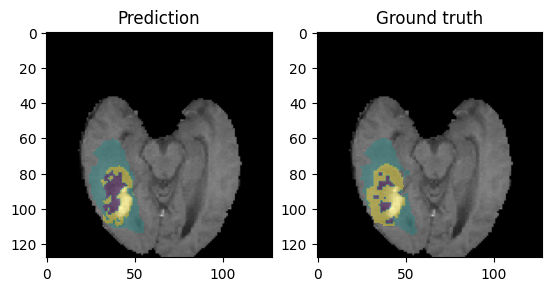
\includegraphics[width=.9\textwidth]{segmentation.png}
	\caption{Links die Segmentierung vom finalen Modell, rechts die wahrhaftige Segmentierung. (Quelle: Eigene Darstellung)}
	\label{fig:segmentation}
\end{figure}
%!TEX root = ../../main.tex
\chapter{Zusammenfassung und Ausblick}
Die vorliegende Studienarbeit hat sich mit dem Einsatz von Deep Learning, insbesondere mit der U-Net-Architektur, für die Segmentierung von Hirntumoren in MRT-Bildern beschäftigt. Durch den Einsatz künstlicher neuronaler Netze konnte eine effektive Methode zur automatisierten Segmentierung vorgestellt werden, die das Potenzial hat, die Diagnostik und Behandlungsplanung in der Neuroonkologie zu verbessern.

Im Rahmen der Arbeit wurden zunächst die theoretischen Grundlagen des Deep Learning und speziell von \ac{CNN} und der U-Net-Architektur erläutert. Die U-Net-Architektur hat sich dabei als geeignet für die Segmentierungsaufgaben in der medizinischen Bildgebung erwiesen. Sie verbindet die Vorteile von Feature-Erkennung und -Lokalisierung, was zu guten Segmentierungsergebnissen führt.

Der verwendete Datensatz, \ac{BraTS}, bietet eine Vielzahl an \ac{MRT}-Bildern mit unterschiedlichen Hirntumoren. Bei der Datenvorverarbeitung wurde auf Aspekte wie Skalierung und Aufteilung eingegangen, um eine optimale Vorbereitung für das Training des neuronalen Netzes zu gewährleisten. Im Zuge der Modellentwicklung wurden verschiedene Hyperparameter evaluiert und eine effiziente Implementierung des Modells vorgestellt.

Die durchgeführten Experimente demonstrieren die Leistungsfähigkeit des Modells. Während die Bewertung der Modelle auf Basis verschiedener Metriken erfolgte, hat die Fehleranalyse wertvolle Einblicke in mögliche Verbesserungen und Optimierungen gegeben.

Der Ausblick auf zukünftige Projekte und Verbesserungen in diesem Bereich ist vielversprechend. Zum einen könnte die Leistung des Modells durch den Einsatz von anderen bzw. moderneren Modellarchitekturen oder verbesserten Trainingstechniken weiter optimiert werden. Zum anderen könnten zusätzliche Datensätze in das Training einbezogen werden, um die Generalisierbarkeit des Modells weiter zu verbessern. Darüber hinaus wäre es interessant, den Einsatz von semi- oder unüberwachtem Lernen zur weiteren Verbesserung der Segmentierungsleistung zu erforschen.

Abschließend kann festgehalten werden, dass trotz der erzielten Ergebnisse und Erfolge in der vorliegenden Arbeit, noch viele weitere Themen und Verbesserungen behandelt werden sollten, im Hinblick auf die Segmentierung von Hirntumoren, um bessere Ergebnisse zu erzielen.


\clearpage

% Bibilography
\cleardoublepage
\printbibliography

% Glossar
\cleardoublepage


% Appendix
\clearpage
\appendix
% !TeX root = ../main.tex

\addchap{\appendixPhrase}




\end{document}
